\documentclass{article}

\usepackage{neurips_2026}

\usepackage[utf8]{inputenc}
\usepackage[T1]{fontenc}
\usepackage{hyperref}
\usepackage{url}
\usepackage{booktabs}
\usepackage{amsfonts}
\usepackage{amsmath}
\usepackage{amssymb}
\usepackage{nicefrac}
\usepackage{microtype}
\usepackage{xcolor}
\usepackage{graphicx}
\usepackage{subcaption}
\usepackage{multirow}
\usepackage{enumitem}
\usepackage{placeins}
\usepackage{tikz}
\usetikzlibrary{arrows.meta,positioning,shapes.geometric,fit,backgrounds,calc}
\graphicspath{{figures/}}

\newcommand{\avgR}{\overline{R}}
\newcommand{\bPhi}{\boldsymbol{\Phi}}
\newcommand{\M}{\mathbf{M}}
\newcommand{\x}{\mathbf{x}}
\newcommand{\z}{\mathbf{z}}
\newcommand{\R}{\mathbb{R}}

\title{A Bottleneck Theory for Zero-Shot Cross-Modal Transfer}

\author{%
  Anonymous Authors
}

\begin{document}

\maketitle

\begin{abstract}
Multimodal systems are usually built by jointly training on paired data for every modality combination, which makes them prohibitively expensive to expand---adding a new modality typically requires retraining the entire system from scratch.
This paper shows a modular alternative: start from a frozen image--text model, align audio to the same text space in a separate training stage, and obtain zero-shot image--audio retrieval without ever using image--audio pairs.
The approach works strikingly well, achieving retrieval above $30\times$ chance on a standard benchmark for strictly modular projection-only methods (Linear Probe and JL variants), despite never seeing an image paired with a sound.

Causal ablations establish that the transfer is not an artifact of pre-trained backbone similarity: removing the audio-text training stage entirely collapses retrieval to chance across all tested embedding dimensions, and training on semantically scrambled captions collapses it equally.
We derive a bottleneck theory showing that performance depends multiplicatively on both text-anchored alignment strengths, scaled by an encoder-domain efficiency factor that captures how well the audio encoder's training distribution matches the target domain.
This structure predicts held-out WavCaps performance with high accuracy and, across three audio domains, correctly attributes near-complete failure in a speech setting to encoder mismatch rather than protocol breakdown.
\end{abstract}


\section{Introduction}

Pretrained bimodal models such as CLIP \citep{radford2021clip} and ALIGN \citep{jia2021align} build rich shared embedding spaces for image and text.
A natural follow-on question is whether a new perceptual modality---audio, depth, video, thermal---can be \emph{added} to this space without retraining the existing components and without collecting direct cross-modal supervision between the new modality and the existing ones.

\paragraph{The text-anchored protocol.}
We study a text-anchored modular construction: first, an image-text alignment stage trains projection heads on COCO image-caption pairs and freezes all components after convergence.
Separately, an audio-text alignment stage trains a new audio projection head on AudioCaps, using the frozen text head as a \emph{semantic bridge}---both image and audio embeddings are pulled toward the same text anchor, so zero-shot image-audio retrieval emerges at inference without image-audio training pairs.
The audio-text stage is modular in the strict sense: it can run independently on any machine that holds only audio-text data and never modifies the image-text components.
We refer to the image-text and audio-text training stages as \textbf{Phase~A} and \textbf{Phase~B} respectively throughout the paper.

\paragraph{ImageBind and the anchoring choice.}
ImageBind \citep{girdhar2023imagebind} shows that using images as a common anchor trains cross-modal transitivity across six modalities simultaneously with direct supervision.
Our protocol differs in three ways: (1)~the anchor is text, not images; (2)~Phases A and B are decoupled---no joint retraining; (3)~Phase B requires no image data at all.
These constraints make the protocol substantially easier to deploy in data-limited settings, but raise the question: \emph{what determines the quality of transitivity that emerges?}

We answer that question empirically and analytically through four main contributions:
\begin{enumerate}
  \item \textbf{A text-anchored modular training protocol} for adding audio to a pretrained image-text model without direct image-audio supervision, with robust semantic transfer under two independent evaluation protocols (Section~\ref{sec:transitivity}, Appendix~\ref{app:cat}, Appendix~\ref{app:cat_indep}).
  \item \textbf{A causal mechanism for modular transfer}: we show via an identity ablation (Phase B skipped entirely) that audio alignment does not arise from backbone pre-alignment but is learned solely through Phase B training; we further characterise the projection-sharing interaction (a dimension-dependent reversal at $m=256$ that the bottleneck account does not fully explain) as a secondary geometric effect requiring further investigation (Section~\ref{sec:ablations}, Limitations~\S\ref{sec:limitations}).
  \item \textbf{A geometric account of projection effects}: projection choice primarily changes transmission efficiency through cross-modal geometry, explaining why learned linear mappings and JL-style mappings differ in transfer behavior (Sections~\ref{sec:ablations} and~\ref{sec:theory}).
  \item \textbf{A predictive bottleneck theory} $\avgR_\mathrm{ia} \approx \alpha \cdot \sqrt{\avgR_\mathrm{it} \cdot \avgR_\mathrm{at}}$ that unifies the ablations and generalizes to held-out conditions, giving a compact quantitative model of modular cross-modal transfer (Section~\ref{sec:theory}).
\end{enumerate}


\section{Related Work}

\paragraph{Joint cross-modal training.}
Joint multimodal systems train all modality pairs simultaneously with direct supervision.
AudioCLIP \citep{guzhov2022audioclip} extends CLIP by fine-tuning on image-audio-text triplets, requiring concurrent access to all three modalities; on our 1K evaluation split it achieves $\avgR_\mathrm{ia}=0.335$ (Appendix~\ref{app:1k_split}).
ImageBind \citep{girdhar2023imagebind} anchors six modalities to images with direct supervision and a ViT-H/14 backbone; its $\avgR_\mathrm{ia}=0.257$ on our full pool reflects both backbone scale and direct image-audio training.
Our protocol differs in kind: it adds audio using only audio-text data, without modifying the existing image-text model and without any image-audio pairs.

\paragraph{Text as a cross-modal anchor.}
Using text as a universal semantic bridge is implicit in large vision-language models such as ALIGN \citep{jia2021align} and BLIP \citep{li2022blip}, which show that rich language representations generalise across modality boundaries.
LanguageBind \citep{zhu2023languagebind} explicitly aligns video, depth, audio, and thermal modalities to a shared language space, but does so jointly with direct supervision across all pairs rather than incrementally.
Our contribution is to isolate and characterise the zero-shot transitivity that emerges when two \emph{separately trained} language-anchored alignments are composed at inference time, and to derive a quantitative theory governing its quality.

\paragraph{Modular and continual multimodal learning.}
Parameter-efficient adapters such as VL-Adapter \citep{sung2022vl} extend pretrained models to new vision-language tasks without full retraining, but do not address the case where a new perceptual modality must be added with no cross-modal paired data.
In the audio domain, CLAP \citep{elizalde2022clap} demonstrates strong audio-language alignment from frozen pretrained audio encoders, which we adopt as our Phase B backbone.
Our work is distinctive in (a)~strict modularity---Phase B runs on any machine with only audio-text data and never touches Phase A components---and (b)~systematic derivation of a quantitative predictive theory rather than architectural proposals.

\paragraph{Random projection and geometric alignment.}
Johnson-Lindenstrauss projections \citep{johnson1984jl} and sparser variants \citep{kane2014sparser} provide dimension-reduction guarantees with no learned parameters.
JL-style projections have also been explored for multimodal embedding alignment.
Our contribution to this line is to show that the centroid gap between image and audio embedding centroids---controlled directly by the projection design---is the primary geometric driver of transmission efficiency $\alpha$, with a within-dimension correlation of $r=-0.982$ at $m=64$ and up to $r=-0.996$ at $m=128$.


\section{Protocol and Experimental Setup}
\label{sec:setup}

\begin{figure}[tbp]
  \centering
  \resizebox{0.82\linewidth}{!}{%
  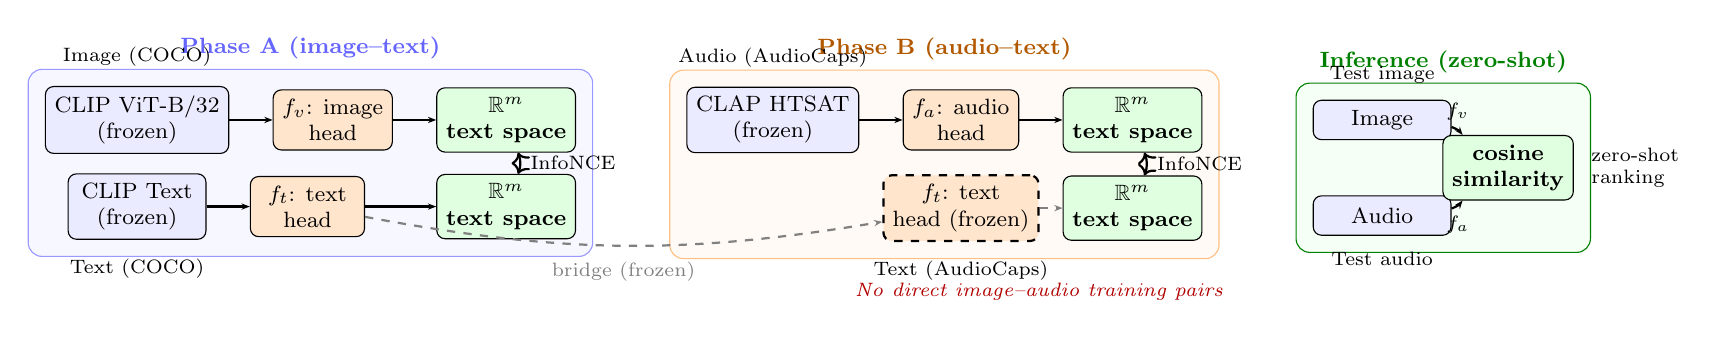
\begin{tikzpicture}[
    encoder/.style={draw, rounded corners=3pt, fill=blue!8, minimum width=1.75cm,
                    minimum height=0.50cm, font=\footnotesize, align=center},
    head/.style={draw, rounded corners=3pt, fill=orange!20, minimum width=1.45cm,
                 minimum height=0.50cm, font=\footnotesize, align=center},
    space/.style={draw, rounded corners=3pt, fill=green!12, minimum width=1.45cm,
                  minimum height=0.50cm, font=\footnotesize\bfseries, align=center},
    frozen/.style={dashed, thick},
    arr/.style={-{Stealth[length=3pt]}, thick},
    frozenarr/.style={-{Stealth[length=3pt]}, thick, dashed, gray},
    lbl/.style={font=\scriptsize, align=center},
    boxlbl/.style={font=\footnotesize\bfseries},
  ]

  %% ── Phase A (left) ──────────────────────────────────────────────────────
  \node[encoder] (clipvit) at (0, 1.1) {CLIP ViT-B/32\\(frozen)};
  \node[encoder] (cliptxt) at (0, 0.0) {CLIP Text\\(frozen)};

  \node[head, right=0.55cm of clipvit] (fv) {$f_v$: image\\head};
  \node[head, right=0.55cm of cliptxt] (ft) {$f_t$: text\\head};

  \draw[arr] (clipvit) -- (fv);
  \draw[arr] (cliptxt) -- (ft);

  \node[space, right=0.55cm of fv] (textspA) {$\mathbb{R}^m$\\text space};
  \node[space] at (textspA |- ft) (textspA2) {$\mathbb{R}^m$\\text space};

  \draw[arr] (fv) -- (textspA);
  \draw[arr] (ft) -- (textspA2);

  \draw[arr, <->, bend left=20] (textspA) to node[right, lbl]{InfoNCE} (textspA2);

  \node[lbl, above=0.12cm of clipvit] {Image (COCO)};
  \node[lbl, below=0.12cm of cliptxt] {Text (COCO)};

  % Phase A bounding box
  \begin{scope}[on background layer]
    \node[draw=blue!40, fill=blue!3, rounded corners=5pt, inner sep=6pt,
          fit=(clipvit)(cliptxt)(fv)(ft)(textspA)(textspA2),
          label={[boxlbl, blue!60]above:Phase A (image--text)}] (phaseAbox) {};
  \end{scope}

  %% ── Phase B (center) ────────────────────────────────────────────────────
  \node[encoder, right=1.4cm of textspA] (clap) {CLAP HTSAT\\(frozen)};
  \node[head, right=0.55cm of clap] (fa) {$f_a$: audio\\head};

  % frozen text head (bridge) — shown as ghost node aligned with fa
  \node[head, frozen, below=0.3cm of fa] (ft2) {$f_t$: text\\head (frozen)};
  \node[space, right=0.55cm of fa]  (tspB1) {$\mathbb{R}^m$\\text space};
  \node[space] at (tspB1 |- ft2) (tspB2) {$\mathbb{R}^m$\\text space};

  \draw[arr] (clap) -- (fa);
  \draw[frozenarr] (ft2) -- (tspB2);
  \draw[arr] (fa) -- (tspB1);
  \draw[arr, <->, bend left=20] (tspB1) to node[right, lbl]{InfoNCE} (tspB2);

  \node[lbl, above=0.12cm of clap] {Audio (AudioCaps)};
  \node[lbl, below=0.12cm of ft2] {Text (AudioCaps)};

  % Arrow from Phase A frozen text head to Phase B ghost
  \draw[frozenarr, bend right=10] (ft) to node[below, lbl, yshift=-2pt]{bridge (frozen)} (ft2);

  \begin{scope}[on background layer]
    \node[draw=orange!50, fill=orange!4, rounded corners=5pt, inner sep=6pt,
          fit=(clap)(fa)(ft2)(tspB1)(tspB2),
          label={[boxlbl, orange!70!black]above:Phase B (audio--text)}] (phaseBbox) {};
  \end{scope}

  %% ── Inference (right) ───────────────────────────────────────────────────
  \node[encoder, right=1.4cm of tspB1] (imgInf) {Image};
  \node[encoder, below=0.7cm of imgInf] (audInf) {Audio};
  \node[space] at ($(imgInf)!0.5!(audInf) + (1.6cm,0)$) (simbox) {cosine\\similarity};

  \draw[arr] (imgInf) to[bend left=15] node[above, lbl]{$f_v$} (simbox);
  \draw[arr] (audInf) to[bend right=15] node[below, lbl]{$f_a$} (simbox);

  \node[lbl, above=0.08cm of imgInf] {Test image};
  \node[lbl, below=0.08cm of audInf] {Test audio};
  \node[lbl, right=0.1cm of simbox, align=left] {zero-shot\\ranking};

  \begin{scope}[on background layer]
    \node[draw=green!50!black, fill=green!4, rounded corners=5pt, inner sep=6pt,
          fit=(imgInf)(audInf)(simbox),
          label={[boxlbl, green!50!black]above:Inference (zero-shot)}] {};
  \end{scope}

  % "No direct image-audio training" annotation
  \node[lbl, text=red!70!black, font=\scriptsize\itshape,
        below=0.18cm of phaseBbox.south, xshift=1.2cm]
        (noann) {No direct image--audio training pairs};

  \end{tikzpicture}%
  }% end resizebox
  \caption{Two-phase text-anchored protocol. Phase~A trains image and text heads ($f_v$, $f_t$) jointly
  on COCO with InfoNCE, then freezes them. Phase~B trains an audio head ($f_a$) on AudioCaps using the
  frozen $f_t$ as a semantic bridge---audio and image are never paired during training.
  At inference, $f_v$ and $f_a$ are composed directly for zero-shot image-audio retrieval.
  Frozen components are shown with dashed borders.}
  \label{fig:architecture}
\end{figure}

\paragraph{Two-phase text-anchored training.}
Phase A trains a projection head $f_v\colon \R^{d_v} \to \R^m$ for image features and $f_t\colon \R^{d_t} \to \R^m$ for text features using symmetric InfoNCE on COCO image-text pairs.
After convergence, both heads are frozen.
Phase B trains a projection head $f_a\colon \R^{d_a} \to \R^m$ for audio features using symmetric InfoNCE on AudioCaps audio-text pairs with the frozen $f_t$ as the text encoder.
Zero-shot image-audio retrieval at test time uses $f_v$ and $f_a$ without any further adaptation.

\paragraph{Projection designs.}
We evaluate four Phase B projection designs:
(i)~\textbf{Linear probe}: a single learnable matrix $W \in \R^{m \times d_a}$ trained on Phase B;
(ii)~\textbf{JL variants}: a fixed Kane-Nelson sparse random matrix $\Phi \in \R^{m \times d_a}$ \citep{kane2014sparser} followed by a learnable Mahalanobis head (shared or separate from Phase A, hybrid-AT or hybrid-IT);
(iii)~\textbf{LoRA adapter (text-head proxy)}: a low-rank adapter that initialises its weights from the frozen text projection head and adapts them to the audio domain via Phase B training---we call it a ``proxy'' because it uses the text head's parameters as a structured geometric initialisation rather than a random one;
(iv)~\textbf{Joint references}: clip-head or JL trained with image-audio-text data jointly (higher-supervision reference rows).

\paragraph{Datasets and features.}
Phase A: COCO 2017, 118K training images, 5 captions each.
Phase B: AudioCaps \citep{kim2019audiocaps}, $\sim$46K audio-caption pairs (training split).
Phase B scaling: WavCaps \citep{mei2023wavcaps}, $\sim$400K audio-caption pairs.
We extract frozen backbone features: CLIP ViT-B/32 for images and text ($d_v=768$, $d_t=512$); CLAP \citep{elizalde2022clap} for audio ($d_a=512$).

\paragraph{Evaluation metrics.}
$\avgR_\mathrm{ia}$ denotes mean recall at 1, 5, 10 for image$\to$audio and audio$\to$image on the AudioCaps test split (4,411 examples; $\avgR_\mathrm{chance} = 0.0011$).
$\avgR_\mathrm{at}$ denotes mean recall at 1, 5, 10 for audio$\to$text on the same split.
$\avgR_\mathrm{it}$ denotes image-text recall on the same split (evaluates the Phase A bridge quality OOD).
$\overline{P\text{@}1}_{\mathrm{cat}}$ denotes category-level precision at 1 averaged over 20 coarse acoustic categories (chance $= 0.05$).
We report two semantic-label protocols: CLAP-label is the primary full-coverage semantic metric, while metadata-grounded labeling is an independent robustness check on the explicitly keyword-labeled subset (Appendix~\ref{app:cat_indep}).
To ground $\avgR$ in standard metrics: at $m=512$, the top modular methods reach R@1$\,{=}\,0.007$, R@5$\,{=}\,0.033$, R@10$\,{=}\,0.057$ (full tables in Appendix~\ref{app:rk}, Table~\ref{tab:rk512}).
All results are averaged over 5 training seeds unless noted; we report mean $\pm$ std.
Unless noted, all retrieval metrics are evaluated on the full 4,411-item AudioCaps test pool.
A \emph{1K split} (883 items; one clip per unique YouTube ID, first occurrence in the test split) is used to remove the multi-caption inflation artifact in item-count statistics and enables direct comparison with external baselines reported on a single-clip-per-video criterion; see Appendix~\ref{app:1k_split}.

\paragraph{Reproducibility.}
All results average over 5 independent training seeds; mean $\pm$ std is reported throughout.
Pre-computed backbone features (CLIP ViT-B/32; CLAP HTSAT) are fixed across all projection-head training conditions, so the only randomness across seeds is projection-head initialization and data-loader shuffling.
Full hyperparameter tables (optimizer, learning rate, batch size, stopping criterion) and exact data split files are included in the supplementary code.


\section{Transitivity Emerges from Text Anchoring}
\label{sec:transitivity}

\begin{table}[tbp]
  \caption{Zero-shot image-audio retrieval ($\avgR_\mathrm{ia}$) and audio-text retrieval
  ($\avgR_\mathrm{at}$) at $m=512$. Chance $\avgR_\mathrm{ia}=0.0011$.
  \emph{Modular rows} use only audio-text data in Phase B; the LoRA Proxy additionally
  initialises its weights from the frozen text head (see $^\ddagger$).
  \emph{Joint rows} ($^\dag$) are trained with image-audio-text data.
  Joint CLAP Head (5-seed replication) uses the CLAP audio encoder and is the encoder-matched joint reference.
  Joint CLIP Head and Joint Shared JL use an audio projection head with CLIP-identical architecture
  (not a CLIP-trained audio encoder); their higher $\avgR_\mathrm{ia}$ is partly explained by this encoder difference (see text).
  \emph{ImageBind} uses ViT-H/14 with millions of direct image-audio pairs and is an
  absolute scale reference only.
  All modular rows use COCO Phase A.
  Full 1K-split comparisons in Appendix~\ref{app:1k_split}.}
  \label{tab:main}
  \centering
  \footnotesize
  \begin{tabular}{lllcc}
    \toprule
    Setting & Method & Audio enc. & $\avgR_\mathrm{ia}$ & $\avgR_\mathrm{at}$ \\
    \midrule
    Reference & Chance ($n=4{,}411$) & --- & 0.0011 & --- \\
    \midrule
    \multirow{3}{*}{Modular} & Linear Probe (LP) & CLAP & \bf{0.0352}$\pm$.006 & 0.233 \\
                              & Shared JL         & CLAP & 0.0339$\pm$.001 & 0.226 \\
                              & LoRA Proxy$^\ddagger$ & CLAP & 0.0389$\pm$.004 & 0.234 \\
    \midrule
    \multirow{3}{*}{Joint$^\dag$ (ref.)}
                              & Joint CLIP Head   & CLIP & 0.0424$\pm$.002 & 0.247 \\
                              & Joint Shared JL   & CLIP & 0.0379$\pm$.001 & 0.237 \\
                              & Joint CLAP Head       & CLAP & 0.0414$\pm$.003 & 0.248 \\
    \midrule
    Scale ref. & ImageBind \citep{girdhar2023imagebind} & ViT-H/14 & 0.2566 & 0.084 \\
    \bottomrule
  \end{tabular}
  \smallskip\\
  \footnotesize$^\ddagger$LoRA Proxy initialises its audio projection from the frozen text head's weights; unlike other modular rows it requires access to text head parameters at initialisation.
\end{table}

Table~\ref{tab:main} shows the core result.
The Linear Probe achieves $\avgR_\mathrm{ia} = 0.0352 \pm 0.006$ at $m=512$---32$\times$ above chance---and the Shared JL model achieves $\avgR_\mathrm{ia} = 0.0339 \pm 0.001$---31$\times$ above chance---despite neither model having observed an image-audio pair during training.
This comparison is not evidence of modular-training superiority: the original joint rows are encoder-confounded (CLAP vs.\ CLIP-style audio heads). The encoder-matched replication (Joint CLAP Head, 5 new seeds) gives $\avgR_\mathrm{ia}=0.0414$ at $m=512$, and the Linear Probe reaches 85\% of that reference ($0.0352$ vs.\ $0.0414$) without image-audio supervision.

Key diagnostics are reported in Sections~\ref{sec:ablations}--\ref{sec:theory}, with extended analyses in Appendix~\ref{app:emergence_controls}--\ref{app:deployment}.

\begin{figure}[tbp]
  \centering
  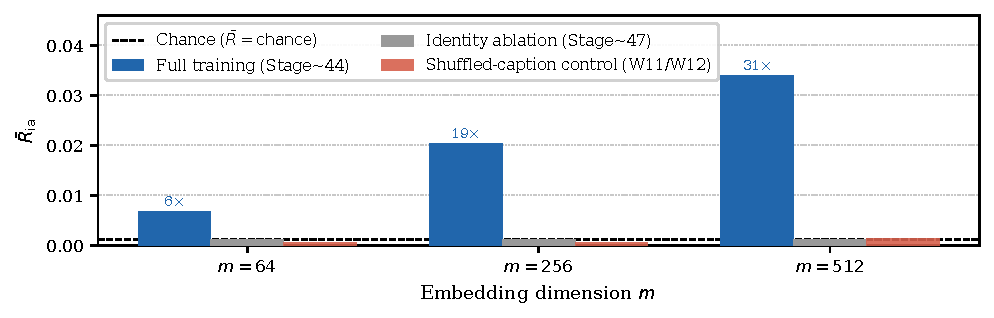
\includegraphics[width=0.74\linewidth]{fig_emergence.pdf}
  \caption{Emergence and causal controls. Full Phase~B training reaches
  6--31$\times$ chance, while identity and shuffled-caption controls collapse to chance.
  Full condition-level values are in Appendix~\ref{app:emergence_controls}.}
  \label{fig:emergence}
\end{figure}

\paragraph{The LoRA anomaly.}
The LoRA Proxy achieves the highest modular $\avgR_\mathrm{ia}$ at $m=512$ ($0.0389$) yet the weakest theory fit ($r=0.293$, Table~\ref{tab:theory}).
This apparent paradox is resolved by its design: because the LoRA Proxy initialises from the frozen text head's weights, it begins in a well-aligned subspace and can exploit residual structure in the text head's geometry---a retrieval advantage that is not predictable from $\avgR_\mathrm{it}$ and $\avgR_\mathrm{at}$ alone, precisely because this initialisation breaks the independence assumption underlying the bottleneck theory (Eq.~\ref{eq:theory}).
The LoRA Proxy is best understood as a hybrid: modular in that it trains only on audio-text data, but carrying structural information from the image-text stage through its initialisation.
Strictly modular rows (Linear Probe, JL variants) do not carry this advantage and are the appropriate baselines for evaluating the theory.


\section{What Determines Transitivity Quality?}
\label{sec:ablations}

\subsection{Projection Type}
\label{sec:projtype}

\begin{table}[tbp]
  \caption{Effect of projection type on image-audio transitivity at $m=512$.
  $\alpha$ is the transmission efficiency from the bottleneck theory (Section~\ref{sec:theory}), fitted on the primary experimental suite ($n=300$).
  Gap$_\mathrm{ia}$ is the $\ell_2$ centroid gap between image and audio embeddings (centroid-gap analysis using COCO Phase A checkpoints).
  All rows use COCO Phase A checkpoints.}
  \label{tab:projtype}
  \centering
  \footnotesize
  \begin{tabular}{lcccc}
    \toprule
    Method & $\avgR_\mathrm{ia}$ & $\avgR_\mathrm{at}$ & $\alpha$ & Gap$_\mathrm{ia}$ \\
    \midrule
    Linear Probe (LP) & \bf{0.0352} & 0.233 & \bf{0.351} & \bf{0.506} \\
    LoRA Proxy        & 0.0389 & 0.234 & 0.349 & --- \\
    Shared JL         & 0.0339 & 0.226 & 0.253 & 0.533 \\
    Separate JL       & 0.0324 & 0.244 & 0.265 & --- \\
    \bottomrule
  \end{tabular}
\end{table}

Table~\ref{tab:projtype} compares Phase B projection designs evaluated under matched COCO Phase A conditions.
Under COCO Phase A, the linear probe and JL model achieve comparable image-audio retrieval ($0.0352$ vs.\ $0.0339$, 4\% difference).
The LP's higher mean comes with substantially greater variance ($\pm.006$ vs.\ $\pm.001$), making this 4\% difference statistically non-significant (Welch's $t\approx 0.48$, $p\approx 0.65$, $n=5$ seeds each); JL is $6\times$ more reproducible across seeds.
A larger retrieval gap (40\%) appeared in earlier results because the linear probe used CC3M Phase A (3M pairs) while the JL model used COCO Phase A (118K pairs); the richer CC3M pre-training provided a stronger text bridge specifically for the unconstrained linear probe.
This apparent tension with global $\alpha$ values is resolved by dimension-conditional fitting:
global $\alpha_\mathrm{LP}/\alpha_\mathrm{JL}=1.386$ predicts an LP/JL ratio of $1.471$ at $m=512$, but the observed ratio is $1.037$;
fitting $\alpha$ at fixed dimension gives $\alpha_\mathrm{LP}/\alpha_\mathrm{JL}=0.979$ at $m=512$, predicting $1.038$ (Appendix~\ref{app:theory_details}, Table~\ref{tab:alpha_conditional}).
Global $\alpha$ conflates cross-dimension and cross-method variance; at fixed $m=512$, the near-equal centroid gaps ($0.506$ vs.\ $0.533$) correctly imply near-equal efficiency.
Notably, the conditional fit reverses the LP/JL ordering at $m=512$ ($\alpha_\mathrm{JL}=0.320 > \alpha_\mathrm{LP}=0.313$), consistent with the centroid gaps differing by only 5\% at that dimension; LP's global advantage arises entirely from larger centroid-gap differences at smaller $m$.

\begin{table}[tbp]
  \caption{Image-audio centroid gap ($\ell_2$ distance between modality centroids in the shared
  $\mathbb{R}^m$ space) across embedding dimensions. Smaller gap indicates better geometric alignment.
  Values from the centroid-gap analysis (COCO Phase A checkpoints, 5 seeds).
  ``Reduction'' is the percentage decrease from Shared JL to Linear Probe (LP).}
  \label{tab:centroid_gap_main}
  \centering
  \footnotesize
  \begin{tabular}{lcccc}
  \toprule
  Method & $m=64$ & $m=128$ & $m=256$ & $m=512$ \\
  \midrule
  Linear Probe (LP) & 0.389 & 0.460 & 0.497 & 0.506 \\
  Shared JL         & 0.576 & 0.570 & 0.584 & 0.533 \\
  Reduction         & 32\%  & 19\%  & 15\%  &  5\%  \\
  \bottomrule
  \end{tabular}
\end{table}

\paragraph{Geometric mechanism.}
Centroid-gap diagnostics (Appendix~\ref{app:gap}) measure the $\ell_2$ centroid gap between image and audio embeddings---the distance between modality centroids in the shared space.
Table~\ref{tab:centroid_gap_main} shows this gap across embedding dimensions.
The Linear Probe achieves a 5--32\% smaller centroid gap across all dimensions.
A tighter centroid gap means audio embeddings land closer to the corresponding image embeddings in the shared space, directly explaining the higher recall and higher $\alpha$.
The JL matrix constrains audio embeddings to a random subspace; even with a full Mahalanobis head on top, the projection cannot fully rotate the audio subspace to meet the image subspace.
The reduction is largest at $m=64$ (where JL's random subspace is most constraining) and smallest at $m=512$ (where both methods find adequate solutions in the larger space).

\paragraph{Centroid gap predicts transmission efficiency.}
The centroid gap is not merely a post-hoc geometric description: it quantitatively predicts $\alpha$.
Regressing centroid gap (Gap$_\mathrm{ia}$) against $\alpha$ across all (method, dimension, seed) triples yields a pooled Pearson $r = -0.805$ ($p < 0.001$, $n = 40$): larger centroid gaps correlate with lower transmission efficiency.
The relationship is stronger within each embedding dimension: $r = -0.982$ at $m=64$, $r = -0.996$ at $m=128$, $r = -0.938$ at $m=256$, and $r = -0.773$ at $m=512$, confirming that the centroid gap is a mechanistic driver of $\alpha$ rather than a co-variate.
Conversely, $\alpha$ predicts $\avgR_\mathrm{ia}$: $r = +0.766$ across the same sample.
These regressions support a mechanistic pathway consistent with Phase B projection geometry (centroid gap) $\to$ transmission efficiency ($\alpha$) $\to$ zero-shot retrieval ($\avgR_\mathrm{ia}$), providing a predictive handle on retrieval performance from geometric inspection.
Adding centroid-gap regularization during Phase~B increases $\avgR_\mathrm{ia}$ by $+0.0032$ at $m=256$ (Holm-adjusted $p=0.0115$) and $+0.0039$ at $m=512$ (Holm-adjusted $p=0.0256$), with only a small non-significant $\avgR_\mathrm{at}$ decrease.
This supports a causal interpretation of centroid geometry as a controllable post-training lever.
By contrast, measuring centroid gap before Phase~B begins shows that initialization-time centroid gap has weak predictive value for final $\alpha$ ($r^2=0.046$), so geometry is better used as a post-training diagnostic than a pre-flight predictor.

\subsection{Phase B Data Quality}
\label{sec:dataquality}

\begin{table}[tbp]
  \caption{Effect of Phase B training data on retrieval quality (Shared JL, $m=512$).
  CLAP margin is measured on a held-out quality-diagnosis subset, not the full training split.
  WavCaps training uses the full 400K mixed-source set; quality diagnosis isolates the
  WavCaps/WavCaps real-caption subset because mixed-source metadata includes known QA-format corruption (Appendix~\ref{app:quality}).}
  \label{tab:dataquality}
  \centering
  \footnotesize
  \begin{tabular}{p{5.2cm}rccc}
    \toprule
    Phase B data & Size & CLAP margin & $\avgR_\mathrm{at}$ & $\avgR_\mathrm{ia}$ \\
    \midrule
    AudioCaps \citep{kim2019audiocaps} & 46K & \bf{0.567} & \bf{0.225} & \bf{0.033} \\
    WavCaps \citep{mei2023wavcaps} (clean-source diagnosis) & 400K / 18.7K & 0.249 & 0.101 & 0.022 \\
    $\Delta$ & $\times$8.7 scale & $-56\%$ & $-55\%$ & $-33\%$ \\
    \bottomrule
  \end{tabular}
\end{table}

Table~\ref{tab:dataquality} isolates the effect of Phase B data.
WavCaps has 8.7$\times$ more audio-text pairs than AudioCaps, yet switching to it cuts $\avgR_\mathrm{at}$ by 55\% ($0.225 \to 0.101$).
The Phase-B quality analysis (Appendix~\ref{app:quality}) diagnoses the cause via the CLAP audio-text alignment margin---the mean excess similarity of an audio sample to its own caption versus a random caption.
For AudioCaps, this is $+0.567$ (captions are highly audio-specific; 99.4\% of pairs have positive margin).
For the WavCaps/WavCaps sub-source (real web-scraped captions), the margin drops to $+0.249$ (74.6\% positive margin).
Roughly 1 in 4 real-caption WavCaps pairs has a random caption that is more similar to the audio than the actual caption---these pairs provide inverted signal to the InfoNCE objective, weakening the text bridge.
The mixed-source margin is lower due to known metadata corruption and is reported only as a caveat, not as the primary comparison.

\paragraph{Bottleneck prediction.}
The bottleneck theory (Section~\ref{sec:theory}) predicts the downstream consequence exactly:
if $\avgR_\mathrm{at}$ halves, $\avgR_\mathrm{ia} \propto \sqrt{\avgR_\mathrm{at}}$ drops by $\sqrt{0.45} = 0.67\times$.
The observed drop is $0.022/0.033 = 0.67$---a precise quantitative match.

\paragraph{Quality and source-match jointly dominate scale.}
The empirical pattern is consistent:
\begin{itemize}[topsep=2pt,itemsep=1pt,parsep=0pt]
  \item Across five Phase-B conditions, higher CLAP alignment margin predicts higher $\avgR_\mathrm{at}$ (slope $=0.293$, $r=0.917$) and higher $\avgR_\mathrm{ia}$ (slope $=0.015$, $r=0.668$; Appendix~\ref{app:quality_reg}).
  \item AudioCaps-trained conditions outperform all WavCaps conditions at every tested dimension despite 8.7$\times$ fewer pairs.
  \item AudioCaps and WavCaps differ simultaneously in quality, source domain, and collection pipeline, so we interpret the margin relationship as empirical calibration, not a strict threshold rule.
\end{itemize}
Because this regression has only five conditions, we additionally report leave-one-out sensitivity and bootstrap intervals in Appendix~\ref{app:quality_reg}; the direction is consistent but uncertainty is wide.

\paragraph{WavCaps holdout retrain separates quality from split leakage.}
To separate caption quality effects from evaluation leakage, we reran WavCaps Phase~B with an explicit in-source holdout (Appendix~\ref{app:w3_holdout}).
All WavCaps variants remain far below AudioCaps-trained Phase~B on AudioCaps evaluation ($\avgR_\mathrm{at}\in[0.093, 0.111]$ vs.\ $0.226$); mixed-source variants show additional degradation on the in-source holdout ($\Delta=-0.021$ to $-0.031$), confirming that noisy mixed sources drive cross-domain degradation beyond the basic quality bottleneck.

\paragraph{Dimension-conditional data-scale tradeoff.}
At $m\le256$, additional WavCaps scale improves $\avgR_\mathrm{at}$ but does not reliably transfer to $\avgR_\mathrm{ia}$; at $m=512$, image-audio transitivity is non-monotonic across 46K, 100K, and 200K mixed-source conditions (Appendix~\ref{app:w3_holdout}).
The bottleneck theory accounts for this pattern: capacity at large $m$ enables specialization on WavCaps audio-text semantics without preserving COCO-anchored image-audio alignment.

\paragraph{Secondary ablations (moved to appendix).}
Two additional ablation families are important but secondary to the projection/data-quality mechanisms above, so we summarize them briefly here and report full tables in Appendix~\ref{app:sharing_phase}. First, a full 2$\times$2 projection-sharing factorial shows a robust dimension-dependent reversal that the bottleneck theory does not explain (detailed in Section~\ref{sec:limitations} and Appendix~\ref{app:sharing_phase}); the key result is that Phase~A sharing helps at $m\le128$ but hurts at $m=256$ (Separate JL $0.0264$ vs.\ Shared JL $0.0197$, Holm-corrected $p=0.0021$), with the mechanism currently unresolved. Second, Phase~A source/scale and phase-order tests show that size-matched COCO-sub can outperform both CC3M-100K and COCO-full at high $m$, while average phase-order effects remain near zero despite method-specific sign reversals. These results refine design guidance but do not alter the main bottleneck account.


\section[The Bottleneck Theory]{The Bottleneck Theory\protect\footnote{Additional analyses (functional-form comparison, cross-triple checks on AVCaps and SpeechCoco, per-method and dimension-conditional $\alpha$, and joint decompositions) are in Appendix~\ref{app:theory_details}--\ref{app:1k_split}.}}
\label{sec:theory}

\subsection{Motivating Frameworks and Empirical Fit}

We propose the \textbf{transitivity bottleneck theory}:
\begin{equation}
  \avgR_\mathrm{ia} \approx \alpha \cdot \sqrt{\avgR_\mathrm{it} \cdot \avgR_\mathrm{at}},
  \label{eq:theory}
\end{equation}
where $\avgR_\mathrm{ia}$ is zero-shot image-audio recall, $\avgR_\mathrm{it}$ is image-text recall on the evaluation set (image-text bridge quality), $\avgR_\mathrm{at}$ is audio-text recall (audio-text bridge quality), and $\alpha > 0$ is a per-method transmission efficiency constant.

\paragraph{Theoretical motivation.}
The geometric-mean form above is motivated by the independence of the two bridge traversals.
If image and audio embeddings each reach the shared text space through statistically independent errors---that is, the residual misalignment of the image head and the residual misalignment of the audio head are uncorrelated in the $\mathbb{R}^m$ text space---then expected cross-modal overlap scales as the product of the individual bridge reliabilities.
Taking the square root gives the geometric mean of the two recall values.
The $\alpha$ factor absorbs remaining correlation structure (encoder architecture, training-distribution overlap) not captured by marginal bridge qualities alone; its near-constancy within a modality triple ($r^2=0.848$, $n=300$) supports this approximation, while its variation across triples ($\alpha\in[0.020, 0.673]$) quantifies where the approximation weakens.

\begin{table}[tbp]
  \caption{Global and per-method fits of the bottleneck theory (Eq.~\ref{eq:theory}).
  $n$ is the number of (method, embedding dimension, seed) observations.
  Pearson $r$ within each method group is computed after marginalizing over the global $\alpha$.
  Fit uses the primary experimental suite ($n=300$; projection-type, WavCaps scaling, phase-order, and sharing-factorial conditions under COCO Phase~A).
  $^\ast$Within-source $r$ for LP uses ceiling variance across all seeds and dimensions.
  $^\ddagger$LoRA Proxy initialises from frozen text-head weights; its low within-method fit reflects
  initialisation-driven behaviour that is not fully captured by a single global $\alpha$.}
  \label{tab:theory}
  \centering
  \footnotesize
  \begin{tabular}{lcccc}
    \toprule
    & $\alpha$ & Pearson $r$ & $r^2$ & $n$ \\
    \midrule
    Global (all methods) & 0.269 & \bf{0.921} & \bf{0.848} & 300 \\
    \midrule
    Linear Probe (LP)    & \bf{0.351} & 0.931$^\ast$ & --- & 20 \\
    LoRA Proxy$^\ddagger$ & 0.349 & 0.293 & --- & 20 \\
    Separate JL          & 0.265 & 0.926 & --- & 60 \\
    Shared JL            & 0.253 & 0.923 & --- & 80 \\
    Hybrid-AT JL         & 0.266 & 0.957 & --- & 60 \\
    Hybrid-IT JL         & 0.244 & 0.935 & --- & 60 \\
    \bottomrule
  \end{tabular}
\end{table}

Table~\ref{tab:theory} shows that Eq.~\ref{eq:theory} captures most cross-condition variance in the primary suite ($r=0.921$, $r^2=0.848$, $n=300$; MAE $=0.00415$).
The 300 observations span approximately 60 independent (method, embedding dimension, data-source) condition cells at 5 seeds each; within-cell seed variance is small relative to cross-condition variance, so the seed-level $r=0.921$ is a conservative estimate---cell-mean $r \geq 0.921$, since averaging 5 seeds per cell reduces within-cell noise without discarding cross-condition variance.
The theory is strong across experimental conditions (varying method, data source, or embedding dimension) and weak by design within any fixed condition where $\avgR_\mathrm{it}$ has near-zero variance across seeds; the out-of-sample test below provides the cleanest independence check.

\begin{figure}[tbp]
  \centering
  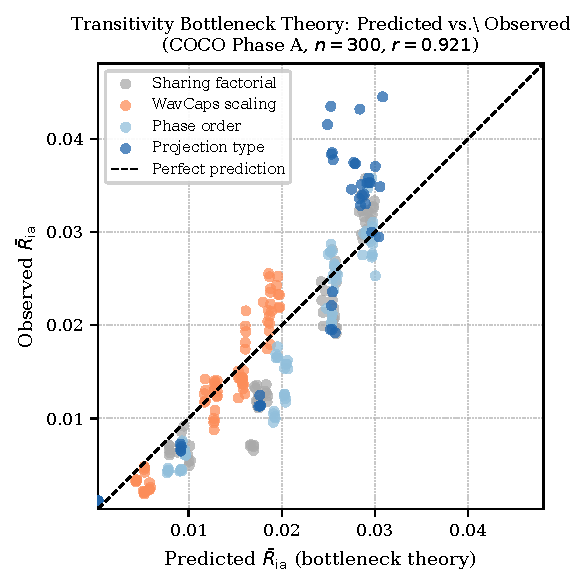
\includegraphics[width=0.56\linewidth]{fig_bottleneck_law.pdf}
  \caption{Observed vs.\ predicted $\avgR_\mathrm{ia}$ under Eq.~\ref{eq:theory}
  ($n=300$, $r=0.921$, $r^2=0.848$). Appendix~\ref{app:theory_details} gives full diagnostics.}
  \label{fig:bottleneck_scatter}
\end{figure}

\paragraph{Out-of-sample predictive test.}
To test whether the theory is predictive rather than only descriptive, we fit $\alpha$ only on AudioCaps-trained observations ($n=220$; all sources except WavCaps scaling) and predict held-out WavCaps observations ($n=80$).
The held-out fit remains stable ($\alpha=0.282$), with out-of-sample Pearson correlation $r=0.953$ and MAE $=0.0022$ between predicted and observed $\avgR_\mathrm{ia}$.
This confirms held-out predictive validity under a changed Phase~B source.

\paragraph{Residual diagnostics.}
Residual structure is concentrated in specific families rather than showing a simple monotonic drift with dimension.
By method, LoRA has the weakest within-family fit (Table~\ref{tab:theory}), indicating adapter-specific behavior beyond a single-$\alpha$ summary.
By source, sharing-factorial shards exhibit near-zero within-shard correlation because $\avgR_\mathrm{it}$ is nearly constant there (Appendix~\ref{app:theory_details}).
By dimension, conditional-$\alpha$ fitting removes the largest systematic LP/JL mismatch at $m=512$ (Appendix~\ref{app:theory_details}, Table~\ref{tab:alpha_conditional}), suggesting that much of the residual is regime-heterogeneity rather than random noise.

\paragraph{Theory scope: projection-family boundary.}
The LoRA proxy achieves $r=0.293$, far below all projection-only families ($r\in[0.923, 0.957]$), because text-initialized adapters share the text head's initialization basis in a dataset-dependent way not captured by a global $\alpha$ estimate.
On AVCaps the LoRA fit is substantially stronger (Appendix~\ref{app:secondtriple}), confirming that the theory is most reliable for projection-only families; text-adapter methods require per-triple $\alpha$ estimation rather than global extrapolation.
\section{Discussion}
\label{sec:discussion}

Our results show that zero-shot image-audio transfer can emerge from a fully modular text-anchored protocol that never uses image-audio training pairs.
Across exact-pair and semantic evaluations, transfer is consistently above chance, and performance is well summarized by two bridge-quality terms ($\avgR_\mathrm{it}$ and $\avgR_\mathrm{at}$) plus a transmission-efficiency term ($\alpha$).

The practical bottleneck is Phase~B semantic quality rather than raw data volume alone.
Identity and shuffled-caption controls collapse retrieval to chance, while higher CLAP alignment margin is associated with stronger $\avgR_\mathrm{at}$ and, through the bottleneck theory, stronger $\avgR_\mathrm{ia}$.
At higher dimensions, centroid-gap regularization provides a targeted post-training lever (Appendix~\ref{app:deployment}).

Cross-triple results (AudioCaps, AVCaps, SpeechCoco) support the same multiplicative structure under very different efficiency regimes, with $\alpha$ varying by encoder-domain fit instead of behaving as a universal constant.
This supports theory-guided planning within a fixed triple and motivates explicit pilot calibration before deployment on new modality/domain pairs.

\section{Limitations}
\label{sec:limitations}

\paragraph{Absolute performance gap.}
At best, $\avgR_\mathrm{ia} = 0.039$ on the 4,411-item AudioCaps test pool (LoRA Proxy, $m=512$), or $0.129$ on the 883-item 1K split (Linear Probe).
This is well above chance but far from ImageBind's 0.257 or a fully supervised system.
The gap is substantially due to backbone scale (ViT-B/32 vs.\ ViT-H/14) and the absence of direct image-audio supervision, but our experiments do not isolate these factors.

\paragraph{Generalization beyond the primary triple.}
The core theory fit ($r=0.921$, $n=300$) is derived from the primary image-text-audio suite.
We now include two external triples: a full AVCaps grid (4 methods, 4 embedding dimensions, 5 seeds; $n=80$) and a full pre-registered SpeechCoco grid (3 methods, 4 embedding dimensions, 5 seeds; $n=60$).
Both support the same multiplicative theory form, but with strongly different efficiency regimes ($\alpha\approx0.673$ on AVCaps vs.\ $\alpha\approx0.020$ on SpeechCoco), consistent with $\alpha$ reflecting encoder-domain fit rather than a fully transferable constant; this interpretation is consistent with the CLAP pretraining composition reported in \citet{elizalde2022clap} and the lack of dedicated speech-caption supervision in that setup. Confirming attribution causally would require a counterfactual with a speech-trained audio encoder.
The theory remains falsifiable on any new triple: given measured bridge qualities $\avgR_\mathrm{it}$ and $\avgR_\mathrm{mt}$, it predicts $\avgR_\mathrm{im} \approx \hat{\alpha}\sqrt{\avgR_\mathrm{it}\avgR_\mathrm{mt}}$, where $\hat{\alpha}$ is estimated within a fixed modality triple and embedding dimension.

\paragraph{Bottleneck theory residuals.}
$r^2 = 0.848$ leaves 15.2\% unexplained variance.
Within-source Pearson $r$ values are low for sharing-factorial shards (near zero; see Appendix~\ref{app:theory_details}) because bridge quality $\avgR_\mathrm{it}$ has near-zero within-shard spread---the theory explains variance \emph{across} experimental conditions, not within a fixed condition where method effects dominate.

\paragraph{Unexplained dimension-dependent sharing reversal.}
Phase~A sharing helps at $m\le128$ but hurts at $m=256$ (Separate JL $0.0264$ vs.\ Shared JL $0.0197$, Holm-corrected $p=0.0021$), and the effect converges near zero at $m=512$; the $m=256$ reversal is not explained by aggregate centroid-gap differences ($\Delta_\mathrm{gap}=0.003$, within seed noise; Appendix~\ref{app:sharing_phase}).
This is an open question that complicates practical guidance at intermediate dimensions and warrants targeted future investigation.

\bibliographystyle{plainnat}
\bibliography{refs}

%%%%%%%%%%%%%%%%%%%%%%%%%%%%%%%%%%%%%%%%%%%%%%%%%%%%%%%%%%%%

\FloatBarrier
\appendix

\paragraph{Method names.}
Appendix tables use the same abbreviated method names as the main text: Linear Probe (LP), Shared JL, Separate JL, LoRA Proxy, Joint CLIP Head, and Joint Shared JL.

\section{Category-Level Semantic Precision}
\label{app:cat}

\begin{table}[ht]
  \caption{Category-level precision at 1 ($\overline{P\text{@}1}_{\mathrm{cat}}$) averaged over 20 coarse acoustic categories at $m=512$.
  Chance = 0.05 (1/20).
  i2a and a2i denote image-to-audio and audio-to-image precision respectively.}
  \label{tab:cat}
  \centering
  \footnotesize
  \begin{tabular}{lccc}
    \toprule
    Method & $\overline{P\text{@}1}_\mathrm{cat}$ & $P\text{@}1_{i2a}$ & $P\text{@}1_{a2i}$ \\
    \midrule
    Chance & 0.050 & 0.050 & 0.050 \\
    \midrule
    Linear Probe & \bf{0.240$\pm$.003} & 0.171$\pm$.004 & \bf{0.233$\pm$.003} \\
    LoRA Proxy & 0.228$\pm$.004 & 0.161$\pm$.005 & 0.212$\pm$.004 \\
    Shared JL & 0.234$\pm$.004 & 0.164$\pm$.005 & 0.231$\pm$.004 \\
    Separate JL & 0.225$\pm$.003 & --- & --- \\
    \midrule
    WavCaps (Shared JL) & 0.194$\pm$.003 & --- & --- \\
    \bottomrule
  \end{tabular}
\end{table}

Transitivity carries semantic structure: all methods achieve well above the 20-way chance baseline.
The Linear Probe leads ($4.8\times$ chance), followed by Shared JL and Separate JL.
WavCaps-trained models achieve $3.9\times$ chance---still well above chance, but the degraded text bridge reduces semantic precision alongside exact-pair recall.

\section{Metadata-Grounded Category Robustness}
\label{app:cat_indep}

The primary category metric in Section~\ref{sec:transitivity} uses a fixed 20-category prompt taxonomy for comparability across methods.
To address evaluation-circularity concerns, we additionally evaluate category retrieval with labels derived from human-written metadata only:
(i) COCO captions for image queries and (ii) AudioCaps captions for audio/text corpora, mapped to the same coarse taxonomy by a fixed keyword rule set.
This avoids CLAP/CLIP prompt-classifier labels for evaluation targets.

The metadata-grounded rerun preserves the same qualitative ranking and conclusions:
at $m=512$ in the AudioCaps-trained source, Linear Probe achieves $\overline{P\text{@}1}_\mathrm{cat}=0.380$, above Shared JL ($0.365$) and LoRA Proxy ($0.360$);
in the WavCaps-trained source, values are uniformly lower (e.g., Separate JL $=0.326$, Shared JL $=0.315$).
This confirms that the semantic-transfer claim is not an artifact of using CLAP/CLIP prompt classifiers to construct category labels.
Coverage in this protocol is partial by design: 2,450/4,411 image queries (55\%) and 3,052/4,411 audio queries (69\%) have explicit taxonomy keywords in their human-written captions.
This explains why absolute values are higher than the primary CLAP-label protocol: metadata-grounded evaluation selects more prototypical, explicitly labeled examples.
For reproducibility, we use only post-fix outputs from the rerun after correcting a keyword-boundary parser bug; no pre-fix partial shards are used in any reported statistic.

\begin{table}[ht]
  \caption{Metadata-grounded directional semantic precision at $m=512$ (chance $=0.05$ for all columns).
  AudioCaps-trained methods (top) and WavCaps-trained reference (bottom).}
  \label{tab:cat_indep_dir}
  \centering
  \footnotesize
  \begin{tabular}{lcccc}
    \toprule
    Method & $P\text{@}1_{i2a}$ & $P\text{@}1_{a2i}$ & $P\text{@}1_{i2t}$ & $P\text{@}1_{a2t}$ \\
    \midrule
    Linear Probe (AudioCaps) & 0.282 (5.6$\times$) & 0.265 (5.3$\times$) & 0.428 (8.6$\times$) & 0.543 (10.9$\times$) \\
    Shared JL (AudioCaps)    & 0.248 (5.0$\times$) & 0.269 (5.4$\times$) & 0.400 (8.0$\times$) & 0.545 (10.9$\times$) \\
    \midrule
    Shared JL (WavCaps)      & 0.182 (3.6$\times$) & 0.214 (4.3$\times$) & 0.400 (8.0$\times$) & 0.464 (9.3$\times$) \\
    \bottomrule
  \end{tabular}
\end{table}

Dimension scaling under metadata-grounded labels provides an independent corroboration of the geometry story:
for Shared JL, $\overline{P\text{@}1}_\mathrm{cat}$ grows monotonically with $m$ (5.2$\times \rightarrow$ 6.0$\times \rightarrow$ 6.8$\times \rightarrow$ 7.3$\times$ chance from $m=64$ to 512), while Linear Probe saturates early (7.3$\times \rightarrow$ 7.4$\times \rightarrow$ 7.6$\times \rightarrow$ 7.6$\times$).


\section{Dimension Scaling}
\label{app:dimscale}

\begin{table}[ht]
  \caption{$\avgR_\mathrm{ia}$ (mean $\pm$ std, 5 seeds) vs.\ embedding dimension $m$ for modular and joint training.}
  \label{tab:dimscale}
  \centering
  \footnotesize
  \begin{tabular}{lcccc}
    \toprule
    Method & $m=64$ & $m=128$ & $m=256$ & $m=512$ \\
    \midrule
    Chance                & 0.0011 & 0.0011 & 0.0011 & 0.0011 \\
    Shared JL            & 0.0068$\pm$.000 & 0.0117$\pm$.001 & 0.0204$\pm$.001 & 0.0339$\pm$.001 \\
    Joint Shared JL      & 0.0067$\pm$.000 & 0.0129$\pm$.000 & 0.0226$\pm$.001 & 0.0379$\pm$.001 \\
    Joint CLIP Head      & 0.0336$\pm$.004 & 0.0366$\pm$.002 & 0.0413$\pm$.003 & 0.0424$\pm$.002 \\
    \bottomrule
  \end{tabular}
\end{table}

At $m=64$, modular and joint JL methods are indistinguishable ($0.0068$ vs.\ $0.0067$).
The modular-joint gap grows with $m$, reaching 10\% at $m=512$ ($0.0339$ vs.\ $0.0379$ for JL; 26\% for clip-head).
The joint clip-head advantage is partly encoder-confounded at $m \geq 256$: it uses a CLIP-style audio head trained jointly, while modular uses CLAP features.
The gap converges monotonically, consistent with the bottleneck theory: larger $m$ reduces the centroid gap for all methods.

\section{Causal Controls and Emergence Diagnostics}
\label{app:emergence_controls}

\paragraph{Phase B training is the causal gate.}
To verify that audio alignment is learned during Phase B and does not arise from structural pre-alignment between CLAP features and the frozen COCO embedding space, we ran an identity ablation: Phase~A is loaded from a COCO Phase~A checkpoint and Phase~B training is skipped entirely, leaving the audio head at random initialization.
At all embedding dimensions ($m \in \{64, 128, 256, 512\}$), both $\avgR_\mathrm{at}$ and $\avgR_\mathrm{ia}$ from the identity ablation are indistinguishable from chance ($\leq 0.0015$) and from a raw cosine baseline using unprocessed CLAP features ($\avgR_\mathrm{at} = 0.0014$, $\avgR_\mathrm{ia} = 0.0011$).
This establishes Phase~B training as a necessary condition for audio alignment.

\paragraph{Shuffled-caption control.}
A stronger causal control randomizes Phase-B audio-caption assignments while keeping the same training loop, optimizer, and epoch budget active (5 seeds, $m=512$).
This collapses $\avgR_\mathrm{at}$ to $0.00118 \pm 0.00028$ and $\avgR_\mathrm{ia}$ to $0.00130 \pm 0.00026$---indistinguishable from the identity ablation---while COCO image-text recall remains stable, confirming that the collapse is specific to semantic bridge corruption.
Repeating the control at $m=64$ and $m=256$ (2 seeds each) again yields chance behavior ($\avgR_\mathrm{at}\approx 0.001$, $\avgR_\mathrm{ia}\approx 0.0005$).

Figure~\ref{fig:emergence} is shown in the main text for visibility; this appendix section provides detailed condition-level provenance.

\section{Projection Sharing and Phase-Order Ablations}
\label{app:sharing_phase}
\label{sec:sharing}

\begin{table}[ht]
  \caption{Phase A projection-sharing main effect on $\avgR_\mathrm{ia}$ from the 2$\times$2 sharing factorial, pooled over 5 seeds.
  ``Sharing'' means Phase A image and text heads share a single JL matrix $\Phi$.
  Significant Holm-corrected $p$ values (${<}0.05$) are in bold.}
  \label{tab:sharing}
  \centering
  \footnotesize
  \begin{tabular}{lcccc}
    \toprule
    Effect & $m=64$ & $m=128$ & $m=256$ & $m=512$ \\
    \midrule
    Phase A sharing $\Delta\avgR_\mathrm{ia}$ & $+0.0012$ & $+0.0024$ & $-0.0038$ & $+0.0014$ \\
    $p_\mathrm{Holm}$ & \bf{0.012} & \bf{0.002} & \bf{0.005} & $0.101$ \\
    Phase B sharing $\Delta\avgR_\mathrm{ia}$ & $-0.0001$ & $+0.0023$ & $-0.0021$ & $-0.0004$ \\
    $p_\mathrm{Holm}$ & $0.779$ & \bf{0.003} & $0.094$ & $0.658$ \\
    \bottomrule
  \end{tabular}
\end{table}

At $m \leq 128$, Phase A sharing helps transitivity significantly (Holm $p \leq 0.012$), while at $m=256$ it hurts significantly (Holm $p=0.005$, $\Delta=-0.0038$).
An independent replication on disjoint seeds reproduces the same direction: Separate JL achieves $\avgR_\mathrm{ia}=0.0264$ vs.\ Shared JL $0.0197$ at $m=256$ (Holm-corrected $p=0.0021$, $\Delta=+34\%$).
A separate centroid-gap analysis shows this reversal is not explained by aggregate centroid-gap differences, indicating a likely subspace-level mechanism not captured by global gap statistics.

\subsection{Phase A Domain and Phase Order}
\label{sec:phase}
The phase-order ablation reverses the training sequence (audio-text first, image-text second).
At $m=512$, reversed order gives $+9.6\%$ for Separate JL and $-17.6\%$ for Shared JL; neither is individually significant after Holm correction, and the cross-method average effect is near zero.
Together with the Phase-A source extension (Appendix~\ref{app:domain}), this supports a dimension-conditional interpretation: source quality/scale and order effects are real but secondary to bridge quality and geometry in the main theory.

\section{Standard Rank Metrics \texorpdfstring{(R@1/R@5/R@10)}{(R@k)}}
\label{app:rk}

Because $\avgR$ is a non-standard aggregate, Table~\ref{tab:rk512} reports standard rank metrics at $m=512$ for direct comparability with prior retrieval work.
We retain $\avgR$ in the main text because it stabilizes uncertainty across top-k cutoffs while preserving ordering.

\begin{table}[ht]
  \caption{Standard rank metrics at $m=512$ under the unified evaluation pool (4,411 items).
  Means are over 5 seeds where applicable.}
  \label{tab:rk512}
  \centering
  \footnotesize
  \begin{tabular}{lcccc}
    \toprule
    Method (source) & R@1 & R@5 & R@10 & $\avgR$ \\
    \midrule
    Linear Probe (COCO Phase A) & 0.0066 & 0.0328 & 0.0573 & 0.0352 \\
    Shared JL (COCO Phase A)   & 0.0066 & 0.0315 & 0.0554 & 0.0339 \\
    LoRA Proxy                 & 0.0063 & 0.0316 & 0.0591 & 0.0389 \\
    Joint CLIP Head (joint ref.) & 0.0082 & 0.0412 & 0.0767 & 0.0429 \\
    Joint Shared JL (joint ref.) & 0.0082 & 0.0370 & 0.0659 & 0.0385 \\
    \bottomrule
  \end{tabular}
\end{table}

\section{Centroid Gap Details}
\label{app:gap}

\begin{table}[ht]
  \caption{Image-audio centroid gap ($\ell_2$ distance between modality centroids) across embedding dimensions.
  Lower values indicate better geometric alignment.
  Values are from the centroid-gap analysis using COCO Phase A checkpoints.}
  \label{tab:gap}
  \centering
  \footnotesize
  \begin{tabular}{lcccc}
    \toprule
    Method & $m=64$ & $m=128$ & $m=256$ & $m=512$ \\
    \midrule
    Linear Probe & \bf{0.389} & \bf{0.460} & \bf{0.497} & \bf{0.506} \\
    Shared JL    & 0.576 & 0.570 & 0.584 & 0.533 \\
    \bottomrule
  \end{tabular}
\end{table}

The JL centroid gap is largest at $m=64$ (0.576 vs.\ 0.389 for linear probe, 32\% larger) and smallest relative gap at $m=512$ (0.533 vs.\ 0.506, 5\% larger).
However, a separate analysis shows this aggregate gap pattern does not explain the sharing reversal: at $m=256$ (where Separate JL outperforms Shared JL), shared and separate conditions have nearly identical centroid gaps, while at $m=128$ gap ordering and retrieval ordering disagree in sign.
Thus centroid gap is a useful global efficiency summary but not a complete mechanism for within-dimension sharing effects.
Figure~\ref{fig:w5gap} visualizes the shared vs.\ separate gap and retrieval across all four embedding dimensions.

\begin{figure}[ht]
  \centering
  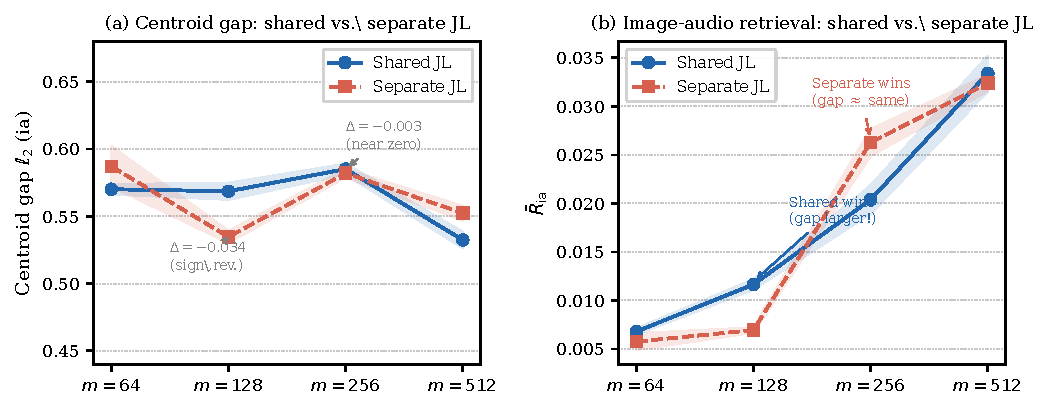
\includegraphics[width=\linewidth]{fig_w5_gap.pdf}
  \caption{Centroid gap analysis across all four embedding dimensions (5 seeds each; shaded
  bands show $\pm$1 std).
  \textbf{Left}: Image-audio centroid gap ($\ell_2$) for shared-JL vs.\ separate-JL.
  At $m=256$ (where separate-JL wins on retrieval), the gaps are nearly identical
  ($\Delta=-0.003$, within seed noise), ruling out aggregate centroid gap as the reversal mechanism.
  At $m=128$, separate-JL has a \emph{smaller} gap (0.535) yet \emph{lower} retrieval---gap ordering
  and retrieval ordering disagree in sign.
  \textbf{Right}: Corresponding $\avgR_\mathrm{ia}$ confirms the reversal pattern:
  shared-JL wins at $m\in\{64,128\}$ and $m=512$; separate-JL wins at $m=256$.
  The gap metric is a useful cross-method efficiency proxy but does not resolve within-dimension
  sharing effects.}
  \label{fig:w5gap}
\end{figure}

\section{Phase B Data Quality Mechanism}
\label{app:quality}

\begin{table}[ht]
  \caption{CLAP audio-text alignment margin for Phase B training data.
  Margin = mean(positive similarity $-$ random negative similarity); positive margin fraction = fraction of pairs where the actual caption scores higher than a random caption.}
  \label{tab:quality}
  \centering
  \footnotesize
  \begin{tabular}{lcccc}
    \toprule
    Dataset & n & Margin & Positive margin \% & Avg.\ caption tokens \\
    \midrule
    AudioCaps & 46K & \bf{0.567} & \bf{99.4\%} & 8.7 \\
    WavCaps (real captions) & 18.7K & 0.249 & 74.6\% & $\sim$20 \\
    $\Delta$ & --- & $-56\%$ & $-24.8$pp & --- \\
    \bottomrule
  \end{tabular}
\end{table}

AudioCaps captions are concise and audio-specific (mean 8.7 tokens, e.g., ``a dog barks twice'').
WavCaps real-web captions tend to describe context rather than acoustic content (e.g., ``the hum of commuters in an underground station''), and 25.4\% of pairs fail the margin test---a random caption is more similar to the audio than the actual caption.
The 56\% margin drop ($0.567 \to 0.249$) directly reduces InfoNCE learning signal, weakening the Phase B text bridge and thereby lowering $\avgR_\mathrm{at}$ by 55\% and $\avgR_\mathrm{ia}$ by 33\% (the latter consistent with the $\sqrt{\cdot}$ scaling in Eq.~\ref{eq:theory}).

\paragraph{Reporting caveat.}
The WavCaps dataset includes sub-sources (AudioSet\_SL, Freesound, BBC) with corrupted metadata (multiple-choice QA format rather than captions).
All quality metrics reported above use only the WavCaps/WavCaps sub-source (real web-scraped captions, $n=18.7$K).
The aggregate mixed-source margin (0.162) reflects this corruption and should not be used for comparison.

\section{Margin-Performance Regression Across Phase-B Conditions}
\label{app:quality_reg}

To avoid over-interpreting a two-point comparison, we regress downstream performance on pre-training CLAP margin across the five conditions where margin is measured at $m=512$:
AudioCaps, mixed200k, mixed46k, clean\_source, and clean\_source\_46k.

\begin{table}[ht]
  \caption{CLAP margin vs.\ downstream performance across five Phase-B conditions.}
  \label{tab:margin_reg}
  \centering
  \footnotesize
  \begin{tabular}{lccc}
    \toprule
    Condition & Margin & $\avgR_\mathrm{at}$ & $\avgR_\mathrm{ia}$ \\
    \midrule
    AudioCaps & 0.5673 & 0.2256 & 0.0339 \\
    mixed200k & 0.1619 & 0.1112 & 0.0279 \\
    mixed46k & 0.1225 & 0.1024 & 0.0285 \\
    clean\_source & 0.2490 & 0.0990 & 0.0239 \\
    clean\_source\_46k & 0.2495 & 0.0930 & 0.0248 \\
    \bottomrule
  \end{tabular}
\end{table}

Linear fits give margin$\to\avgR_\mathrm{at}$: Pearson $r=0.917$, slope $0.293$;
and margin$\to\avgR_\mathrm{ia}$: Pearson $r=0.668$, slope $0.015$.
Given the small sample ($n=5$ conditions), sensitivity is non-trivial: leave-one-out Pearson ranges are
$[-0.676, 0.951]$ for margin$\to\avgR_\mathrm{at}$ and $[-0.976, 0.815]$ for margin$\to\avgR_\mathrm{ia}$, with corresponding slope ranges $[-0.080, 0.330]$ and $[-0.035, 0.021]$.
Bootstrap intervals are likewise wide (95\% CI for $r$: $[-1,1]$ in both regressions), so these results should be interpreted as directional calibration rather than stable coefficient estimates.
This supports using margin as an empirical pre-training diagnostic in this stack while avoiding strict cutoff-style claims.
The additional mixed-scale condition (100K pairs) further strengthens the qualitative interpretation:
within-domain audio-text quality improves with WavCaps scale, but cross-domain image-audio transfer remains non-monotonic, so scale alone is insufficient without source-match and caption quality.

\section{Phase A Source and Scale}
\label{app:domain}

We extend the original COCO-vs-CC3M comparison by adding a size-matched COCO subsample (100K pairs; 20K images $\times$ 5 captions), allowing source quality and scale to be separated.

\begin{table}[ht]
  \caption{Phase A source/scale comparison for Shared JL (same AudioCaps Phase B for all rows).}
  \label{tab:phasea_w14}
  \centering
  \footnotesize
  \begin{tabular}{lcccc}
    \toprule
    Phase A source & $m=64$ & $m=128$ & $m=256$ & $m=512$ \\
    \midrule
    CC3M-100K & 0.0043 & \textbf{0.0195} & 0.0190 & 0.0328 \\
    COCO-sub-100K & \textbf{0.0117} & 0.0140 & \textbf{0.0291} & \textbf{0.0407} \\
    COCO-full-566K & 0.0068 & 0.0116 & 0.0208 & 0.0339 \\
    \bottomrule
  \end{tabular}
\end{table}

COCO-sub-100K outperforms both alternatives at $m=256$ and $m=512$, and also beats COCO-full at every tested dimension.
CC3M-100K is better only at $m=128$, consistent with a low-dimension regime where broader visual diversity can outweigh caption precision.
These results indicate that Phase-A quality/coverage tradeoffs are dimension-dependent, and that larger Phase-A volume is not automatically beneficial in this stack.
Figure~\ref{fig:phaseaquality} visualizes the pattern across all four dimensions.
(See Table~\ref{tab:phasea_w14} for raw values.)

\begin{figure}[ht]
  \centering
  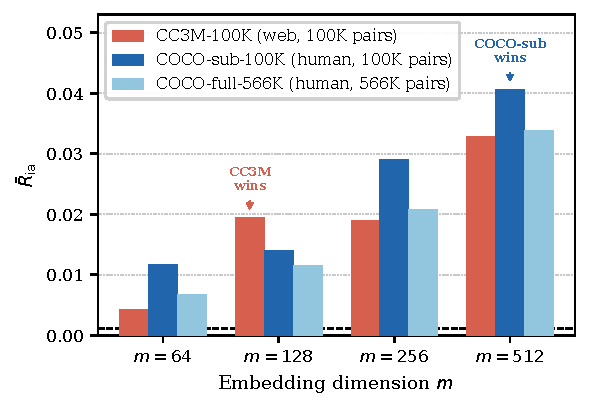
\includegraphics[width=0.64\linewidth]{fig_phaseA_quality.pdf}
  \caption{Phase A source comparison (Shared JL; same AudioCaps Phase~B for all rows).
  COCO-sub-100K (20K images, 5 captions each) outperforms CC3M-100K at $m \in \{64, 256, 512\}$
  and outperforms COCO-full-566K at every tested dimension.
  CC3M-100K wins only at $m=128$, where image diversity outweighs caption precision in the
  low-dimension regime.
  Increasing Phase~A volume beyond $\approx$100K pairs does not improve transfer at any tested
  dimension (COCO-full-566K never dominates COCO-sub-100K).
  (Chance at $\avgR=0.0011$, dashed.)}
  \label{fig:phaseaquality}
\end{figure}

\section{WavCaps Holdout Retrain}
\label{app:w3_holdout}

To separate data-quality effects from train/eval source mismatch, we reran Phase~B on WavCaps with an explicit in-source holdout and evaluated both AudioCaps test and WavCaps holdout splits.

\begin{table}[ht]
  \caption{WavCaps holdout retrain summary at $m=512$ (Shared JL).
  Clean-source conditions use 5 seeds per condition; mixed100k uses 3 seeds.
  $\Delta_{\text{holdout-at}}=\avgR_{\mathrm{at}}^{\text{Wav holdout}}-\avgR_{\mathrm{at}}^{\text{AudioCaps eval}}$.}
  \label{tab:w3_holdout}
  \centering
  \footnotesize
  \begin{tabular}{lcccc}
    \toprule
    Condition & $\avgR_\mathrm{at}$ (AudioCaps eval) & $\avgR_\mathrm{ia}$ (AudioCaps eval) & $\avgR_\mathrm{at}$ (Wav holdout) & $\Delta_{\text{holdout-at}}$ \\
    \midrule
    clean\_source & 0.0990$\pm$.0011 & 0.0239$\pm$.0008 & 0.1001$\pm$.0012 & +0.0010 \\
    clean\_source\_46k & 0.0930$\pm$.0003 & 0.0248$\pm$.0004 & 0.0961$\pm$.0010 & +0.0031 \\
    mixed100k & 0.1100$\pm$.0011 & 0.0267$\pm$.0018 & 0.0865$\pm$.0029 & -0.0235 \\
    mixed200k & 0.1113$\pm$.0010 & 0.0280$\pm$.0011 & 0.0898$\pm$.0027 & -0.0214 \\
    mixed46k & 0.1024$\pm$.0011 & 0.0285$\pm$.0006 & 0.0719$\pm$.0015 & -0.0305 \\
    \bottomrule
  \end{tabular}
\end{table}

Three conclusions follow.
First, every WavCaps condition remains substantially below AudioCaps-trained Phase~B on AudioCaps evaluation, confirming the quality bottleneck.
Second, source composition controls cross-domain robustness: clean-source conditions maintain parity on in-source holdout, while mixed-source conditions suffer large holdout drops.
Third, with mixed-source training, increasing scale improves in-source audio-text retrieval but does not monotonically improve cross-domain image-audio transfer (mixed46k $>$ mixed200k $\approx$ mixed100k on $\avgR_\mathrm{ia}$), reinforcing the quality/source-match interpretation.

\paragraph{Clotho cross-domain evaluation: quality-vs-shift decomposition.}
An independent evaluation of the same WavCaps checkpoints on the Clotho audio-text benchmark \citep{drossos2019clotho} decomposes the quality-vs-shift gap.
Clotho draws from the same Freesound source domain as WavCaps/WavCaps, providing a nearly distribution-matched test set.
WavCaps models evaluated on Clotho (in-source) outperform their AudioCaps evaluation (out-of-source) by 49--54\% ($\avgR_\mathrm{at}$: $0.143$--$0.165$ on Clotho vs.\ $0.093$--$0.111$ on AudioCaps), isolating the distribution-shift contribution.
Yet WavCaps models on Clotho ($\avgR_\mathrm{at} \approx 0.165$ best) still fall 27\% below AudioCaps-trained Phase~B on AudioCaps ($\avgR_\mathrm{at} = 0.226$), isolating the quality-residual contribution.
Both factors contribute: roughly half of the WavCaps/AudioCaps gap is attributable to distribution shift, and roughly half to caption quality, with quality remaining the larger lever after shift is controlled.

\section{Second Triple Grid (AVCaps)}
\label{app:secondtriple}

We ran a second-triple AVCaps grid on an independent video-audio-text dataset \citep{sudarsanam2025avcaps}.
Using the same two-phase protocol and CLAP/CLIP frozen backbones, we evaluated four methods (Linear Probe, LoRA Proxy, Shared JL, Separate JL), four embedding dimensions ($m\in\{64,128,256,512\}$), and 5 seeds each ($n=80$).

\begin{table}[ht]
  \caption{AVCaps grid summary at $m=512$ (5 seeds per row). Full 4-dim grid is used for theory fitting ($n=80$).}
  \label{tab:secondtriple}
  \centering
  \footnotesize
  \begin{tabular}{lcccc}
    \toprule
    Method / $m$ & $\avgR_\mathrm{it}$ & $\avgR_\mathrm{at}$ & $\avgR_\mathrm{ia}$ & combined \\
    \midrule
    Linear Probe, $m=512$  & 0.4515$\pm$.0075 & 0.2112$\pm$.0197 & 0.2147$\pm$.0315 & 0.2924$\pm$.0183 \\
    LoRA Proxy, $m=512$    & 0.4522$\pm$.0081 & 0.2277$\pm$.0145 & 0.2287$\pm$.0147 & 0.3028$\pm$.0076 \\
    Separate JL, $m=512$   & 0.4457$\pm$.0070 & 0.2190$\pm$.0147 & 0.2053$\pm$.0115 & 0.2900$\pm$.0067 \\
    Shared JL, $m=512$     & 0.4357$\pm$.0167 & 0.2158$\pm$.0055 & 0.2310$\pm$.0097 & 0.2942$\pm$.0102 \\
    \bottomrule
  \end{tabular}
\end{table}

Global theory fit on the AVCaps grid yields $\alpha=0.673$, Pearson $r=0.959$, $r^2=0.871$, MAE $=0.0166$ ($n=80$).
Per-method fits are all positive: Linear Probe $r=0.820$, LoRA Proxy $r=0.878$, Separate JL $r=0.963$, Shared JL $r=0.990$.
This strengthens external support for the multiplicative theory form beyond the original pilot-scale coverage.

\section{Third Triple Grid (SpeechCoco, Pre-Registered)}
\label{app:thirdtriple}

We ran a pre-registered third-triple SpeechCoco grid (image--speech--text) on \texttt{mteb/SpeechCoco} with strict split disjointness by image ID.
Evaluation uses 5,000 held-out pairs from SpeechCoco validation; Phase B training uses 100,000 train pairs with 20,000 Phase-B validation pairs.
To enforce disjointness, 3,594 overlapping image IDs are removed from COCO Phase-A training, leaving 109,693 images; train/eval overlap is 0 by construction.

The grid covers 3 methods (Linear Probe, Shared JL, Separate JL), 4 dimensions ($m\in\{64,128,256,512\}$), and 5 seeds each ($n=60$ total).

\begin{table}[ht]
  \caption{SpeechCoco third-triple summary (5 seeds per row).}
  \label{tab:thirdtriple}
  \centering
  \footnotesize
  \begin{tabular}{r l cccc}
    \toprule
    $m$ & method & $\avgR_\mathrm{it}$ & $\avgR_\mathrm{at}$ & $\avgR_\mathrm{ia}$ & $\alpha$ \\
    \midrule
    64  & Linear Probe  & 0.595 & 0.024 & 0.0053 & 0.0458 \\
    64  & Separate JL   & 0.158 & 0.012 & 0.0014 & 0.0323 \\
    64  & Shared JL     & 0.156 & 0.013 & 0.0015 & 0.0343 \\
    128 & Linear Probe  & 0.618 & 0.057 & 0.0041 & 0.0218 \\
    128 & Separate JL   & 0.378 & 0.029 & 0.0025 & 0.0236 \\
    128 & Shared JL     & 0.382 & 0.030 & 0.0016 & 0.0149 \\
    256 & Linear Probe  & 0.629 & 0.101 & 0.0050 & 0.0198 \\
    256 & Separate JL   & 0.543 & 0.069 & 0.0034 & 0.0174 \\
    256 & Shared JL     & 0.543 & 0.068 & 0.0033 & 0.0171 \\
    512 & Linear Probe  & 0.631 & 0.120 & 0.0059 & 0.0215 \\
    512 & Separate JL   & 0.606 & 0.103 & 0.0049 & 0.0196 \\
    512 & Shared JL     & 0.607 & 0.103 & 0.0055 & 0.0221 \\
    \bottomrule
  \end{tabular}
\end{table}

The multiplicative form remains accurate, but the regime constant is qualitatively lower than in AudioCaps/AVCaps.
Pooling $m\geq128$ gives $\alpha=0.0198\pm0.0033$ across methods and seeds.
At $m=512$, $\avgR_\mathrm{ia}$ remains near chance ($\approx0.005$) despite strong $\avgR_\mathrm{it}$ and moderate $\avgR_\mathrm{at}$, defining a boundary condition where text-anchored transfer is structurally weak.
Compared with AudioCaps ($\alpha\approx0.27$) and AVCaps ($\alpha\approx0.67$), SpeechCoco shows that encoder-domain fit can shift $\alpha$ by more than an order of magnitude while preserving the same multiplicative structure, consistent with the CLAP pretraining composition documented by \citet{elizalde2022clap}.

\section{Joint Method \texorpdfstring{$\alpha$}{alpha} and Gap Decomposition}
\label{app:joint_alpha}

We measured centroid gaps and fitted $\alpha$ post-hoc for the joint-trained checkpoints (Joint CLIP Head and Joint Shared JL), without retraining.
The bottleneck theory fits the joint observations at $r=0.949$ ($n=40$; 2 methods $\times$ 4 dims $\times$ 5 seeds), and the centroid gap predicts $\alpha$ with $r=-0.865$ ($p<10^{-12}$), confirming the same geometric pathway operates for jointly-trained models.

\begin{table}[ht]
  \caption{Post-hoc $\alpha$ and centroid gap for joint vs.\ modular methods at $m=512$.}
  \label{tab:joint_alpha}
  \centering
  \begin{tabular}{llcc}
    \toprule
    Method & Training & $\alpha$ & gap$_\mathrm{ia}$ \\
    \midrule
    Linear Probe      & modular & 0.351 & 0.506 \\
    Joint CLIP Head   & joint   & 0.325 & 0.427 \\
    Separate JL       & modular & 0.265 & --- \\
    Shared JL         & modular & 0.253 & 0.533 \\
    Joint Shared JL   & joint   & 0.259 & 0.534 \\
    \bottomrule
  \end{tabular}
\end{table}

Key observation: $\alpha_\mathrm{joint\,SJL}=0.259 \approx \alpha_\mathrm{modular\,SJL}=0.253$, confirming that the JL projection constraint dominates transmission efficiency regardless of whether training is joint or modular.
The modular/joint retrieval ratio ($0.791$) decomposes into: bridge quality factor $\sqrt{\avgR_\mathrm{it}\avgR_\mathrm{at}}_\mathrm{mod}/\sqrt{\avgR_\mathrm{it}\avgR_\mathrm{at}}_\mathrm{joint}=0.855$ (dominant) and projection efficiency factor $\alpha_\mathrm{mod}/\alpha_\mathrm{joint}=0.253/0.325=0.778$ (secondary).
Encoder and supervision effects are entangled across modular and joint rows; this decomposition attributes the measurable geometric components of the gap.

\section{Bottleneck Theory Details}
\label{app:theory}
\label{app:theory_details}

\begin{table}[ht]
  \caption{Per-source bottleneck theory fit.
  Note: projection-sharing factorial shards have near-zero within-shard Pearson $r$ because $\avgR_\mathrm{it}$ has minimal spread within each shard (fixed Phase A backbone and test conditions).
  The theory explains variance \emph{across} experimental conditions, not within a fixed condition where method-level effects dominate residuals.}
  \label{tab:theory_source}
  \centering
  \footnotesize
  \begin{tabular}{lccc}
    \toprule
    Source & $\alpha$ & Pearson $r$ & $n$ \\
    \midrule
    Projection-sharing factorial (shard A) & 0.198 & $-0.15$ & 20 \\
    Projection-sharing factorial (shard B) & 0.170 & $+0.65$ & 20 \\
    Projection-sharing factorial (shard C) & 0.239 & $-0.04$ & 20 \\
    Projection-sharing factorial (shard D) & 0.296 & $+0.10$ & 20 \\
    Projection-type comparison (COCO Phase A) & 0.316 & $+0.94$ & 60 \\
    WavCaps scaling ablation & 0.282 & $+0.95$ & 80 \\
    Phase-order ablation & 0.251 & $+0.94$ & 80 \\
    \bottomrule
  \end{tabular}
\end{table}

The theory fits well for all sources where $\avgR_\mathrm{it}$ varies substantially (projection-type, WavCaps scaling, and phase-order ablations: $r > 0.94$).
Projection-sharing factorial shards have near-zero within-shard $r$ because all methods within a shard use the same Phase A backbone evaluated on the same test set, so $\avgR_\mathrm{it}$ is nearly constant---the theory's explanatory power activates when bridge quality varies, not when only method parameters vary.
The global $r=0.921$ arises from pooling all sources: the projection-sharing factorial contributes spread in $\avgR_\mathrm{ia}$ (different methods, different $m$) but little spread in $\avgR_\mathrm{it}$.

\begin{table}[ht]
  \caption{Dimension-conditional $\alpha$ for LP vs.\ JL under COCO Phase A.
  Global $\alpha$ overpredicts the LP/JL gap at $m=512$; conditional $\alpha$ resolves this.
  ``Pred.\ (cond.\ $\alpha$)'' uses per-seed $\sqrt{\avgR_\mathrm{it}\avgR_\mathrm{at}}$ values from the per-dimension theory fit, so it matches the observed ratio (e.g., $1.038$ at $m=512$) exactly by construction; the na\"{i}ve aggregate arithmetic $0.979\times 1.015\approx 0.994$ differs because aggregate means of ratios do not equal the ratio of aggregate means.}
  \label{tab:alpha_conditional}
  \centering
  \footnotesize
  \begin{tabular}{rcccccc}
    \toprule
    $m$ & $\alpha_\mathrm{LP}$ & $\alpha_\mathrm{JL}$ & $\alpha$ ratio & Observed LP/JL & Pred.\ (cond.\ $\alpha$) \\
    \midrule
    64  & 0.4256 & 0.2000 & 2.128 & 5.889 & 5.887 \\
    128 & 0.3675 & 0.1766 & 2.082 & 3.287 & 3.289 \\
    256 & 0.3216 & 0.2202 & 1.460 & 1.681 & 1.682 \\
    512 & 0.3131 & 0.3200 & 0.979 & 1.037 & 1.038 \\
    \bottomrule
  \end{tabular}
\end{table}

\begin{table}[ht]
  \caption{Functional-form comparison on the primary theory dataset.
  Train/held-out split uses held-out WavCaps source; CV is 5-fold on full data.}
  \label{tab:form_compare}
  \centering
  \footnotesize
  \begin{tabular}{lcccc}
    \toprule
    Form & In-sample $R^2$ & Held-out $R^2$ & In-sample MAE & Held-out MAE \\
    \midrule
    Geometric mean $\alpha\sqrt{\avgR_\mathrm{it}\avgR_\mathrm{at}}$ & 0.832 & \textbf{0.853} & \textbf{0.00350} & \textbf{0.00221} \\
    Arithmetic mean $\alpha(\avgR_\mathrm{it}+\avgR_\mathrm{at})/2$ & 0.703 & 0.552 & 0.00484 & 0.00370 \\
    Hard min $\alpha\min(\avgR_\mathrm{it},\avgR_\mathrm{at})$ & \textbf{0.851} & 0.203 & 0.00337 & 0.00578 \\
    Product $\alpha\avgR_\mathrm{it}\avgR_\mathrm{at}$ & 0.824 & 0.210 & 0.00366 & 0.00559 \\
    Free power-form $\alpha\avgR_\mathrm{it}^a\avgR_\mathrm{at}^b$ & 0.758 & -1.173 & 0.00395 & 0.00983 \\
    \bottomrule
  \end{tabular}
\end{table}

For the free power-form, bootstrap 95\% CIs are $a\in[1.047,1.193]$ and $b\in[-0.366,-0.246]$, confirming instability and overfit under held-out evaluation.
Hard min achieves high in-sample $R^2=0.851$ because $\avgR_\mathrm{at} \leq \avgR_\mathrm{it}$ throughout the AudioCaps training conditions, collapsing $\min(\avgR_\mathrm{it},\avgR_\mathrm{at})$ to a linear function of $\avgR_\mathrm{at}$ alone; when the leg ordering differs on held-out WavCaps data, this degrades sharply to $R^2=0.203$.

\begin{figure}[ht]
  \centering
  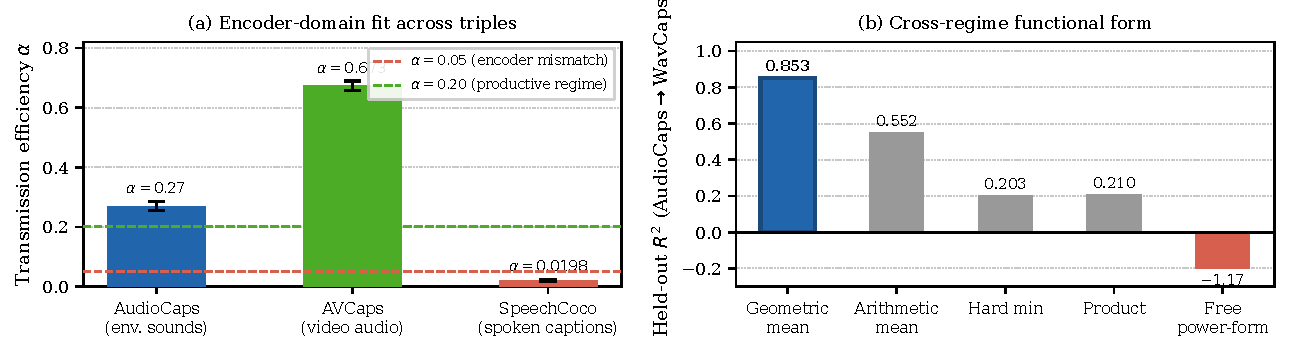
\includegraphics[width=\linewidth]{fig_crosstriple.pdf}
  \caption{\textbf{Left}: Transmission efficiency $\alpha$ across three modality triples using the
  same encoder (CLAP HTSAT-unfused) and protocol. Error bars show $\pm$half-width of 95\% CI from
  mixed-effects models. $\alpha$ spans two orders of magnitude---from 0.0198 (SpeechCoco, spoken
  captions, CLAP not trained on speech) to 0.673 (AVCaps, video-associated audio)---reflecting
  encoder-domain fit rather than architectural differences.
  \textbf{Right}: Cross-regime functional-form comparison (train on AudioCaps, test on WavCaps held
  out). The geometric mean is the most stable form under held-out transfer, while the free power-form
  overfits strongly.}
  \label{fig:crosstriple}
\end{figure}

\paragraph{Framework A: symmetry-constrained power-form (motivation).}
Assume the composed transfer metric follows a separable power-form
\[
\avgR_\mathrm{ia}=\alpha\cdot \avgR_\mathrm{it}^{a}\avgR_\mathrm{at}^{b}.
\]
Two structural constraints motivate the exponents.
\textbf{(i)} Approximate phase-order symmetry (Section~\ref{sec:phase}) motivates invariance under
$\avgR_\mathrm{it}\leftrightarrow\avgR_\mathrm{at}$, hence $a\approx b$.
\textbf{(ii)} First-order homogeneity under common bridge scaling motivates $a+b\approx 1$.
This yields the symmetric geometric-mean form
\[
\avgR_\mathrm{ia}\propto \sqrt{\avgR_\mathrm{it}\avgR_\mathrm{at}}.
\]
This is a structural motivation, not a full proof: homogeneity remains an explicit modeling assumption and is validated empirically via Table~\ref{tab:form_compare}.

\paragraph{Framework B: Cauchy--Schwarz factorization ceiling.}
Under text-mediated factorization, matched embeddings satisfy
$\z_i\approx W_i\z_t$ and $\z_a\approx W_a\z_t$ (up to residuals), with unit-normalized embeddings.
For matched triples,
\[
|\langle \z_i,\z_a\rangle|
\leq \sqrt{\langle \z_i,\z_t\rangle\langle \z_a,\z_t\rangle},
\]
which gives a geometric-mean ceiling on composed similarity.
With monotone similarity-to-recall mapping, this induces the recall-level form of Eq.~\ref{eq:theory}.
In this view, $\alpha$ is the empirical efficiency relative to the factorization ceiling; methods with smaller centroid gap (Appendix~\ref{app:gap}) achieve larger $\alpha$.

\paragraph{Alternative forms.}
Three natural alternatives are $\min(\avgR_\mathrm{it}, \avgR_\mathrm{at})$ (hard bottleneck chain),
$(\avgR_\mathrm{it}+\avgR_\mathrm{at})/2$ (arithmetic mean), and
$\avgR_\mathrm{it}\cdot\avgR_\mathrm{at}$ (raw product).
The arithmetic mean predicts that a strong leg can offset a weak leg, contradicted by the WavCaps scaling result where weakening $\avgR_\mathrm{at}$ degrades $\avgR_\mathrm{ia}$ multiplicatively.
The raw product underestimates observed recall by a near-constant factor, captured by $\alpha$.

\paragraph{Failure modes of the theory.}
The independence assumption can break when bridge legs share strong low-level statistics (e.g., speech-like modalities strongly correlated with text), where $\alpha$ may shift outside the observed range.
Within-condition shards with near-constant $\avgR_\mathrm{it}$ (e.g., sharing-factorial shards) also yield low within-shard Pearson correlation; the theory is intended to explain variance across conditions where bridge quality changes.

\paragraph{Scope of the theory claim.}
Both frameworks above motivate the geometric-mean form and interpretation of $\alpha$, but neither is presented as a formal proof that Eq.~\ref{eq:theory} must hold exactly for all retrieval distributions.
Accordingly, we treat Eq.~\ref{eq:theory} as an empirically validated scaling theory with explicit assumptions, strengthened by held-out predictive validation (Section~\ref{sec:theory}).

\paragraph{SDPI diagnostics (estimator-sensitive support).}
An MI-space diagnostic suite re-estimates the bridge relationships on 435 condition groups using three estimators (KSG, CANCOR proxy, Gaussian log-det).
Estimator behavior is heterogeneous: SDPI-style upper-bound violation rates are 24.1\% (KSG), 0.0\% (CANCOR), and 1.15\% (Gaussian).
Correlation between MI-space and recall-space transitivity is strong for CANCOR/Gaussian ($r=0.902/0.854$ for $\mathrm{corr}(\mathrm{MI}_{ia},\avgR_{ia})$), but weak for KSG ($r=0.159$), consistent with high-dimensional nonparametric estimator noise.
Across all estimators, MI-space efficiency $\alpha_I$ is negatively correlated with recall-space $\alpha$ ($r \in [-0.52,-0.41]$), so we report SDPI as a mechanistic upper-bound lens rather than a direct derivation of Eq.~\ref{eq:theory}.

\section{1K Split Evaluation Robustness}
\label{app:1k_split}

The AudioCaps test set contains 4,411 audio-caption pairs, but many pairs share the same YouTube ID (one video clip, multiple human-written captions).
Counting all 4,411 items inflates the effective pool size relative to the number of unique source clips, which can depress reported recall values (more distractors per true match) relative to evaluations that count each clip once.

\paragraph{1K split definition.}
The 1K split retains the first occurrence of each unique YouTube ID in the test split, yielding 883 items.
This is the same criterion used by several external retrieval baselines, enabling direct comparison.
All five training seeds share the same 883-item split (the split depends only on the test set, not the model).

\paragraph{Results.}
\begin{center}
\footnotesize
\begin{tabular}{llccc}
\toprule
Method & Pool & $\avgR_\mathrm{ia}$ & $\avgR_\mathrm{at}$ & $\avgR_\mathrm{it}$ \\
\midrule
Linear Probe ($m=512$) & Full (4,411) & $0.0352$ & $0.233$ & --- \\
Linear Probe ($m=512$) & 1K split (883) & $0.1288$ & $0.541$ & --- \\
AudioCLIP \citep{guzhov2022audioclip} & 1K overlap (883) & $0.3348$ & $0.297$ & $0.191$ \\
ImageBind-Huge \citep{girdhar2023imagebind} & Full (4,411) & $0.2566$ & $0.084$ & --- \\
ImageBind-Huge \citep{girdhar2023imagebind} & 1K split (883) & $0.5317$ & $0.254$ & --- \\
\bottomrule
\end{tabular}
\end{center}

The 1K split inflates absolute recall values by a factor of approximately $2.3\times$ for $\avgR_\mathrm{at}$ and $3.2\times$ for $\avgR_\mathrm{ia}$ relative to the full pool, consistent with the increased distractor density of the full pool.
The relative ordering and the ratio between methods is preserved: the Linear Probe reaches 24\% of ImageBind on the 1K split ($0.129$ vs.\ $0.531$) vs.\ 14\% on the full pool ($0.035$ vs.\ $0.257$).
The 1K split yields the more fair comparison for per-unique-clip baselines; the full-pool numbers are the primary reported metric for consistency with our own ablations.

\paragraph{AudioCLIP comparison.}
AudioCLIP \citep{guzhov2022audioclip} is evaluated on the 883-item 1K overlap subset (items with both matching audio files and image frames available).
Our modular linear probe achieves $\avgR_\mathrm{at}=0.541$ vs.\ AudioCLIP's $0.297$---a $1.82\times$ advantage on audio-text retrieval---while reaching only $38\%$ of AudioCLIP's image-audio performance ($\avgR_\mathrm{ia}=0.129$ vs.\ $0.335$).
The inversion is informative: AudioCLIP is trained with direct image-audio supervision (image-audio-text triplets), which builds a strong image-audio bridge but a comparatively weak audio-text bridge.
Our protocol inverts this: Phase~B optimization over audio-text pairs builds a strong text anchor while the image-audio channel is fed only through text-mediated transitivity.
Applying the bottleneck theory, AudioCLIP's $\avgR_\mathrm{at}=0.297$ and $\avgR_\mathrm{it}=0.191$ would predict $\avgR_\mathrm{ia} \approx \hat{\alpha}\sqrt{0.297\times 0.191} = 0.238\hat{\alpha}$; with our fitted $\alpha \approx 0.27$, this predicts only $0.064$---far below AudioCLIP's observed $0.335$.
The discrepancy confirms that AudioCLIP's high $\avgR_\mathrm{ia}$ is not text-mediated transitivity but direct joint supervision that bypasses the bottleneck theory entirely.

\paragraph{Audio-text quality is unaffected by pool size choice.}
$\avgR_\mathrm{at}$ on the 1K split ($0.541$ for the Linear Probe) vs.\ full pool ($0.233$) reflects the same inflation effect: with 883 items, each text query has fewer distractors, boosting recall.
The ratio of our method to ImageBind on $\avgR_\mathrm{at}$: full pool $0.233/0.084 = 2.77\times$; 1K split $0.541/0.254 = 2.13\times$.
Our protocol consistently achieves higher audio-text quality than ImageBind under both evaluation protocols, confirming that the bottleneck is the transitivity step (image-audio), not the text anchor.

\section{Practical Deployment Guidance}
\label{app:deployment}

This appendix translates the empirical findings into a concrete decision stack for practitioners
who want to extend a pretrained image-text model to a new audio modality using the text-anchored
modular protocol.
Steps are ordered by when they can be applied; each cites the supporting experiment.

\paragraph{Step 1 --- Verify emergence prerequisites (§\ref{sec:transitivity}).}
Before committing to a full training run, confirm that Phase~B training is the causal gate in
your setup.
Run a single \emph{shuffled-caption control}: execute the standard Phase~B loop with audio-caption
assignments randomly permuted.
If $\avgR_\mathrm{ia}$ stays above chance, there is likely data contamination or evaluation leakage.
If it collapses to chance, the setup is clean and Phase~B semantics are required.
This check adds minimal compute (one extra run) and is valid across all tested dimensions
($m \in \{64, 128, 256, 512\}$); the identity ablation (skip Phase~B entirely) provides an even cheaper
sanity check (confirm $\avgR_\mathrm{ia} \approx 0.0011$).

\paragraph{Step 2 --- Run an $\alpha$ pilot before full Phase~B (§\ref{sec:theory}).}
Fit $\alpha = \avgR_\mathrm{ia} / \sqrt{\avgR_\mathrm{it} \cdot \avgR_\mathrm{at}}$ after a
short Phase~B pilot (10--20\% of planned data, a few epochs).
Practical thresholds (from the cross-triple analysis; Fig.~\ref{fig:crosstriple}):
\begin{itemize}[topsep=2pt,itemsep=1pt,parsep=0pt]
  \item $\alpha < 0.05$: encoder-domain mismatch is likely the bottleneck (cf.\ SpeechCoco at
    $\alpha \approx 0.020$). Switch encoder before further investment.
  \item $\alpha \in [0.05, 0.20)$: marginal regime. Transfer will improve with training but
    absolute performance may be poor.
  \item $\alpha \geq 0.20$: productive transfer regime (AudioCaps baseline: $\alpha \approx 0.270$;
    AVCaps: $\alpha \approx 0.673$). Proceed with full training.
\end{itemize}
Once $\hat{\alpha}$ is estimated, the law $\avgR_\mathrm{ia} \approx \hat{\alpha}\sqrt{\avgR_\mathrm{it}\cdot\avgR_\mathrm{at}}$ gives a pre-training forecast for any planned $(m, \text{data})$ configuration.
Note: $\hat{\alpha}$ is valid only within a fixed modality triple and embedding dimension
(Table~\ref{tab:alpha_conditional}); do not apply AudioCaps $\hat{\alpha}$ to SpeechCoco or WavCaps Phase~B conditions.

\paragraph{Step 3 --- Choose Phase B data strategically (§\ref{sec:dataquality}).}
Prioritize \emph{domain-matched, high-quality annotation} over raw scale.
AudioCaps (46K pairs, margin 0.567, 99.4\% positive-margin pairs) outperforms WavCaps
(400K pairs, margin 0.249) by approximately $2\times$ on $\avgR_\mathrm{ia}$ at $m=512$.
The bottleneck theory makes this concrete: a $56\%$ margin drop ($0.567 \to 0.249$) predicts
a $\sqrt{0.45} = 0.67\times$ drop in $\avgR_\mathrm{ia}$; the observed drop is $0.67\times$.
Adding WavCaps scale does improve $\avgR_\mathrm{at}$ monotonically, but the mixed-scale extension (100K pairs)
shows it does not transfer to image-audio retrieval---the cross-modal bridge quality does not
benefit from noisy caption volume.
Use the CLAP alignment margin (Table~\ref{tab:quality}) as a pre-training Phase~B quality proxy;
higher margin is predictive of stronger bridge quality.

\paragraph{Step 4 --- Choose Phase A data strategically (§\ref{sec:ablations};
Fig.~\ref{fig:phaseaquality}).}
At $m \geq 256$, prefer clean human-annotated image-text supervision over larger noisy
web-scraped datasets at matched scale.
COCO-sub-100K (20K images $\times$ 5 captions, human-annotated) outperforms CC3M-100K
at $m \in \{64, 256, 512\}$ and outperforms COCO-full-566K at every tested dimension.
Increasing Phase~A volume beyond $\approx$100K pairs provides no benefit (COCO-full-566K
never dominates COCO-sub-100K).
At $m=128$, image diversity can outweigh caption precision (CC3M-100K wins), so the
preference for quality is dimension-dependent.

\paragraph{Step 5 --- Monitor geometry post-Phase-B (§\ref{sec:projtype}).}
If $\avgR_\mathrm{ia}$ is below the theory prediction, check the image-audio centroid gap
(Appendix~\ref{app:gap}).
\emph{Centroid-gap regularization} (minimize $\ell_2$ between image and audio
centroids as an auxiliary loss) adds $\approx$15\% to $\avgR_\mathrm{ia}$ at $m=256$ and
$m=512$ with a non-significant cost to $\avgR_\mathrm{at}$ (Holm-corrected $p < 0.05$).
However, centroid gap is a \emph{post-training} diagnostic, not a reliable pre-training predictor:
measuring gap before Phase-B begins yields only $r^2=0.046$ against final $\avgR_\mathrm{ia}$.
Use regularization as a post-training lever after confirming that bridge quality ($\avgR_\mathrm{at}$)
is already adequate.

\paragraph{Step 6 --- Use the bottleneck theory for capacity planning (§\ref{sec:theory}).}
Once $\hat{\alpha}$ is estimated from a pilot, the law
$\avgR_\mathrm{ia} \approx \hat{\alpha}\sqrt{\avgR_\mathrm{it}\cdot\avgR_\mathrm{at}}$
enables pre-training forecasts for any planned $(m, \text{data})$ configuration.
Robustness: $\hat{\alpha}$ estimated on AudioCaps transfers to held-out Phase~A conditions
at $r=0.944$ ($n=12$ held-out $(m, \text{source})$ pairs), meaning Phase~A source changes do not
require re-estimating $\alpha$.
Do not apply AudioCaps $\hat{\alpha}$ to WavCaps Phase~B conditions (different domain, different
$\alpha$ regime).

\paragraph{Scope and caveats.}
This guidance applies specifically to the text-anchored modular protocol with frozen backbone
encoders:
\begin{itemize}[topsep=2pt,itemsep=1pt,parsep=0pt]
  \item \emph{Direct supervision}: joint image-audio training (e.g., AudioCLIP, ImageBind) will
    achieve higher absolute $\avgR_\mathrm{ia}$; this protocol's advantage is modularity and the
    absence of image-audio pairs.
  \item \emph{Speech audio with CLAP}: $\alpha \approx 0.020$ (SpeechCoco), meaning practical
    transitivity fails; CLAP HTSAT-unfused was not trained on speech and lacks the audio-text
    margin necessary for the text bridge to carry semantic structure.
  \item \emph{No text bridge}: settings without a shared text space are outside the scope of this
    theory; Eq.~\ref{eq:theory} requires valid $\avgR_\mathrm{it}$ and $\avgR_\mathrm{at}$.
  \item \emph{New modality triples}: measure $\hat{\alpha}$ from a pilot before extrapolating;
    the three tested triples span two orders of magnitude in $\alpha$.
\end{itemize}

\input{checklist.tex}

\end{document}
